%*****************************************************************************************
%*********************************** Second Chapter **************************************
%*****************************************************************************************

\chapter{Excitons in lead iodide perovskites}

\graphicspath{{Chapter2/Figures/}}

\section{Properties of excitons}
In an ideal crystal, the orbitals of a periodic array of atoms $\sim$\AA\,s apart overlap, and instead of discrete atomic energy levels, we instead find energy bands due to mixing between atomic levels. We can think of the resulting electron bands using two models: either by starting with a free conduction electron gas then adding the perturbation from the periodic potential of the ionic atomic cores (Bloch's theorem), or by adding weak interactions between the overlapping neutral atoms so electrons can hop between atomic sites (tight binding approximation, similar to linear combination of atomic orbital approach). In general this is complicated many-body problem, with both electron-electron and electron-core interactions to take into account in the Hamiltonian of the system, as well as the motions of carriers. Such a problem cannot be solved analytically, and requires computing power in order to calculate the band structure of even simple solids. The interactions mean the electron dispersion deviates from the free electron value of $E=\frac{\hbar^2k^2}{2m_e}$ where $E$ is the energy of the electron, $k$ the wavevector of the electron wavefunction, related to its momentum $p$ by $p=\hbar k$, and $m_e$ is the rest mass of a free electron.

However we can still use some basic trends to describe the behaviour of charge carriers in solids. The most important energy bands are the valence band (VB), the highest band occupied by electrons (\textit{c.\,f.\,}highest occupied molecular orbital in molecules), and the conduction band (CB), the lower non-occupied band (\textit{c.\,f.\,}lowest unoccupied molecular orbital). The gap between the highest point of VB and lowest point of CB is known as the band gap $E_g$; when this gap occurs at the same $k$ point the material is said to have a direct band gap, and if not the band gap is indirect. The behaviour of free carriers depends on the relative energies of these bands with respect to the Fermi energy ($E_F$), defined as the energy of the energy of the highest occupied state at 0\,K [Fig.\,\ref{2Fig1}(a)]. Conduction depends on the availability of free electrons in the CB, where there are free states for electrons to move into. If $E_F$ is within the VB (i.\,e.\,VB and CB overlap), then the solid is a metal. If $E_F$ is in the gap between the VB and CB, then the material is a semiconductor if $E_g$ is small ($\lesssim1$\,eV) so that electrons can be thermally excited to the CB, or an insulator if $E_g$ is larger. Also as a result of electrons, the mass of an electron $m_e$ is no longer given by the free electron rest mass value. Instead is depends on the curvature of the energy band, and the `effective electron mass' of the electron $m_e^{*}$ when responding to forces depends on the dispersion of the band it occupies as
\begin{equation}
\centering
m_e^{*} = \frac{\hbar^2}{\frac{d^2E}{dk^2}} .
\label{effectivemass}
\end{equation}
For the rest of the Chapter we will drop the effective mass label * for brevity, however it should be noted that in general the free electron mass is only an approximation to the actual crystal value.

When electrons are excited from the VB they leave behind `holes', quasiparticles used to describe an absence of electrons with a charge of $+e$, $k_h = -k_e$ and $m_h \approx m_e$ although this depends on the dispersion of the energy bands in question. The attraction between the electron and hole binds them together to form a hydrogen-like neutral particle in the crystal. We can therefore use results from the hydrogen atom to find the binding energy $E_B$ and Bohr radius $a_B$:
\begin{subequations}
\label{ex3D}
\begin{align}
E_B &=\frac{\mu e^4}{32\pi^2\epsilon^2\epsilon_0^2\hbar^2n^2} = \frac{R_H}{n^2}\frac{\mu}{\epsilon^2 m_e} \label{exbinding3D}\\
a_B &= \frac{4\pi\epsilon\epsilon_0\hbar^2}{\mu e^4}=a_0\frac{\epsilon m_e}{\mu} \label{exrad3D},
\end{align}
\end{subequations}
where $\mu = (\frac{1}{m_e}+\frac{1}{m_h})^{-1}$ is the effective mass of the exciton, $\epsilon$ is the dielectric constant of the material, and $n$ is the energy level of the exciton, with $n=1, 2, 3...$. The Rhydberg constant $R_H=13.6$\,eV, and most probably distance between a proton and electron in the ground state $a_0=0.5$\,\AA are defined with respect to the hydrogen atom. Due to $E_B$, exciton energies have energies below free electrons in the CB, and form a series of hydrogenic level below the lower edge of the CB [Fig.\,\ref{2Fig1}(b)]. The energy of an exciton $E_{ex}$ is given by
\begin{equation}
\centering
E_{ex} = E_g - E_B + \frac{\hbar^2}{2M}(k_x^2+k_y^2+k_z^2),
\label{exenergy}
\end{equation}
where $M = m_e+m_h$ is the total mass of the exciton, and the $k_i$ terms describe its motion in 3D. Eq.\,\ref{exenergy} gives the energy of free electrons that are able to move throughout the crystal, however excitons can be bound to impurities, further lowering their energy.

Mott-Wannier excitons typically exist in inorganic materials, where high $\epsilon$ gives rise to $E_B \sim 10$\,eV and $a_B \sim 100$\,\AA. Therefore such excitons extend over many unit cells, and due to low $E_B$ low temperature measurements are required to observe Mott-Wannier excitons optically, although we can often observe multiple $n$ states [Fig.\,\ref{2Fig1}(c)]. Conversely Frenkel excitons general exist in organic materials with low $\epsilon$, so $E_B \sim 1$\,eV and $a_B \sim 10$\,\AA. Frenkel excitons are limited to a few unit cells, or in the case of molecular organic semiconductors, the same molecule. If the charge carriers can hop between molecular sites then such excitons are known as charge-transfer excitons.
\begin{figure}[ht] 
\centering    
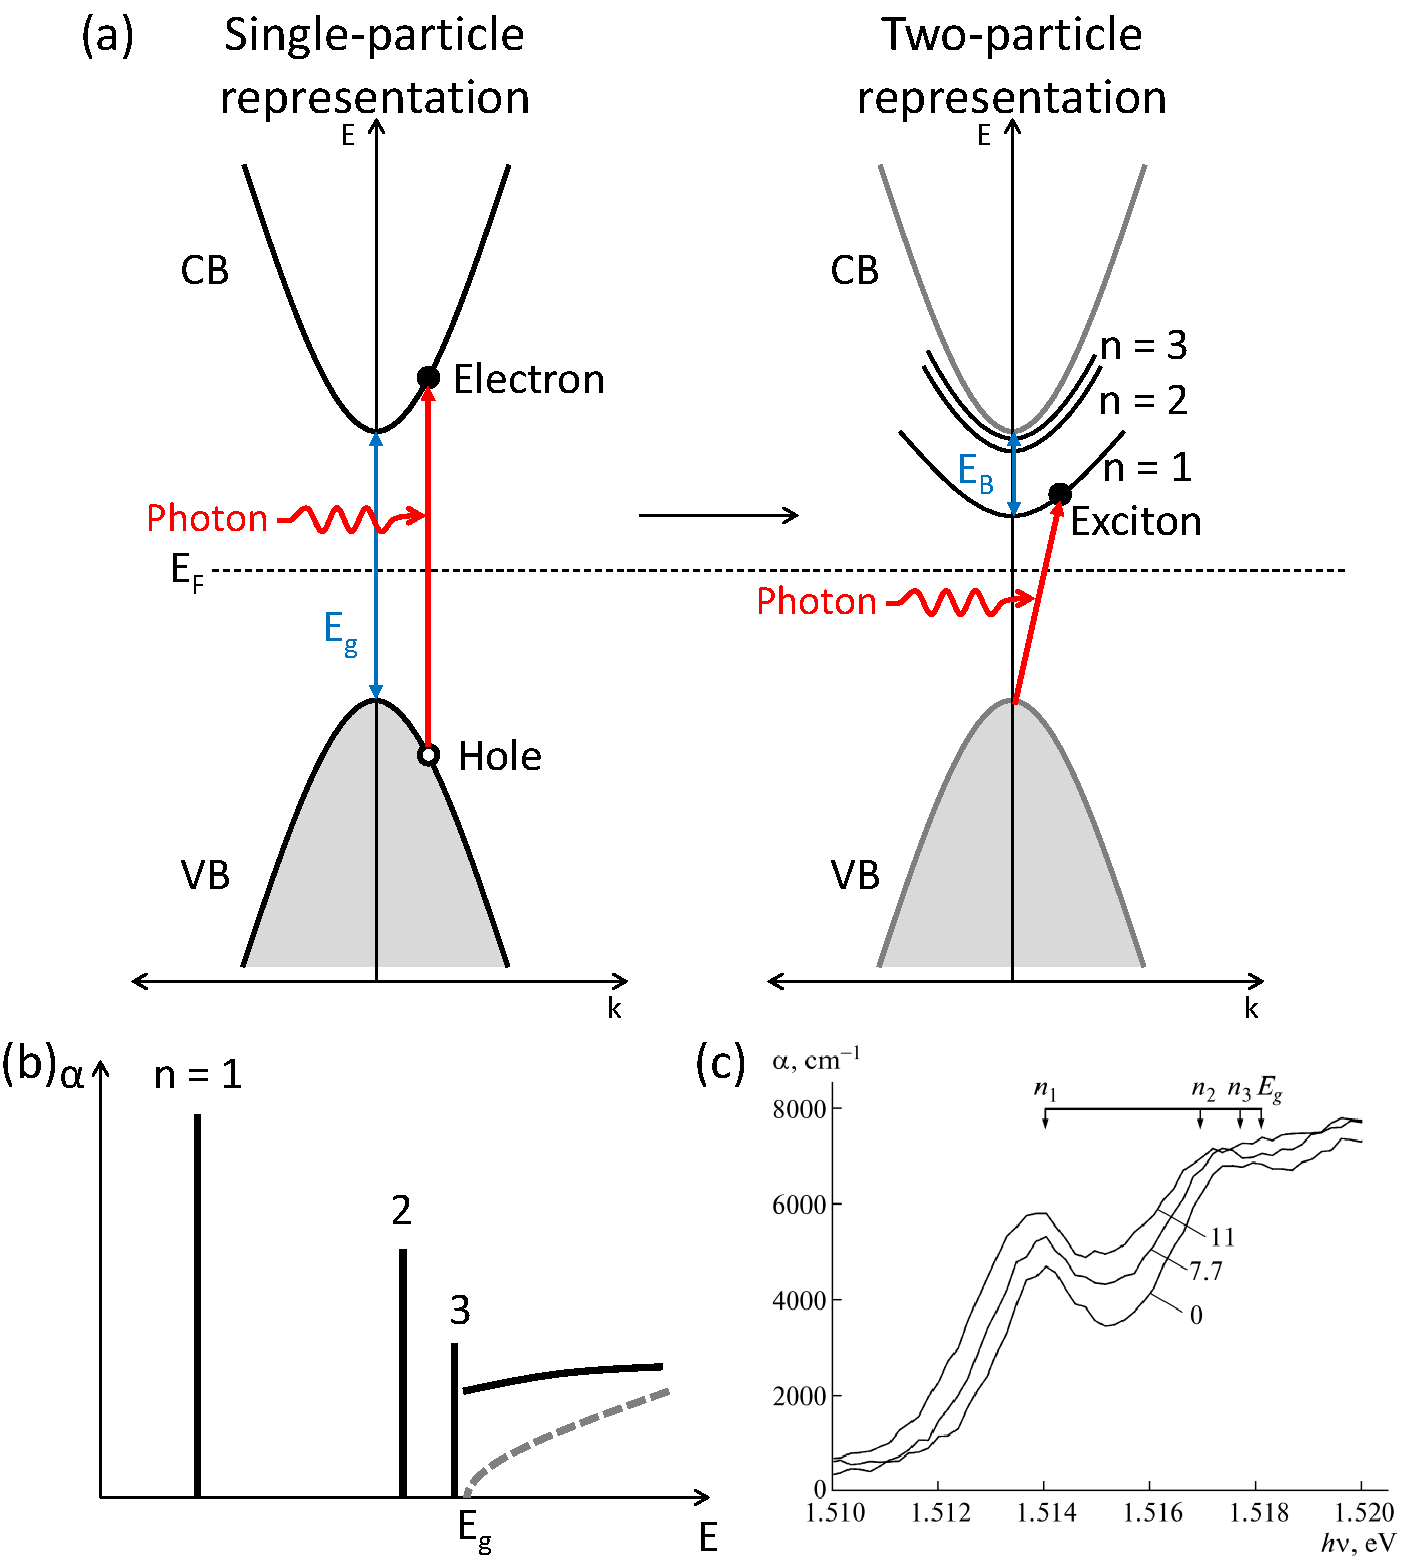
\includegraphics[width=\textwidth]{Fig1}
\caption{(a) Schematic of band structures of insulators, semicnoductors and metals. (b) Schematic of exciton bands below the conduction band. (c) Theoretical absorption spectrum of a 3D semiconductor according to Eq.\,\ref{exabs} (not to scale). The dotted line shows the expected band edge absorption without the Sommerfeld factor (see text). (d) Experimental absorption spectrum of GaAs crystal at 1.7\,K, with the labelled laser power (W/cm$^2$). From Ref.\,\cite{Vaganov2013}.}
\label{2Fig1}
\end{figure}

As mentioned previously, excitons can be created by the absorption of a photon. In bulk semiconductors, the absorption coefficient $\alpha$ depends on the initial ground state $\ket{i}$ of a filled VB and empty CB and final state $\ket{f}$ of one promoted electron as
\begin{equation}
\centering
\alpha = \left| \Braket{f | i} \right|^2 \rho(E) ,
\label{exabs}
\end{equation}
where the matrix element $\braket{f | i}$ gives rise to selection rules of possible electronic transitions, and the joint density of states $\rho(E)$ is the number of states per unit energy range between the CB and VB at the photon energy $E$. In 3D $\rho(E)$ has a $\sqrt{E-E_g}$ dependence, however in experiment the Coulomb interaction leads to an enhancement in the absorption by the Sommerfeld factor, and $\alpha$ is not discontinuous at zero at $E_g$ as expected from Eq.\,\ref{exabs} \cite{Bassu1997}. This gives rise to the theoretical absorption spectrum shown in Fig.\,\ref{2Fig1}(c), with discrete exciton absorption lines decreasing in intensity as $n^{-3}$ \cite{Bassu1997}, and continuous absorption at higher energy due to interband transitions. 

One difference between the theoretical and measured absorption spectrum is due to the overlap of the exciton lines and band edge absorption as a result of the finite width of exciton peaks ($\Gamma_{ex}$). The finite exciton width is due to a number of factors: firstly homogeneous variable that affect each exciton equally, such as the radiative lifetime of the exciton ($\frac{1}{\Gamma_{ex}(0)}$), and collisions with phonons. Secondly inhomogeneous factors such as impurities ($\Gamma_{imp}$), whose effects will be more localised. Overall this leads to a measured linewidth $\Gamma_{ex}$ that varies with temperature $T$ as
\begin{equation}
\centering
\Gamma_{ex}(T) = \Gamma_{ex}(0) +  \Gamma_{imp}(T) +A_{ac}T + \frac{B_{op}}{\exp{\frac{\hbar\omega_p}{k_B T}}-1},
\label{exwidth}
\end{equation}
where the contribution to phonon collision can be separated into coupling with acoustic phonons ($A_{ac}$), and interactions with polarised optical phonons of energy $\hbar\omega_p$ \cite{Dammak2009}. 

Once excitons are excited via absorption, they can also emit that energy in the form of a photon. Thus in emission spectra the strength of exciton peaks depends also on the oscillator strength $f$, given by the matrix element between the exciton and photon wavefunctions. The strong coupling between excitons and photons also gives rise to exciton-polaritons. The non-propagating exciton solution at $k=0$ gives rise to the longitudinal exciton-polariton frequency $\omega_L$, while the travelling plane-wave solution gives rise to the transverse exciton-polariton with frequency $\omega_T$ as $k\rightarrow \infty$. The absorption of a photon to form the charged constituents of an exciton causes deformation of the crystal, and as a result of the structural rearrangement the annihilation of the exciton causes emission of a photon at a lower energy. This is known as the Stokes shift, which has a larger value for Frenkel excitons in organic semiconductors due to the more easily deformed molecules.

\section{Excitons in 2D systems}
Exciton motion can be confined to 2D is quantum well (QW) systems, where a material with smaller $E_g$ (well) is sandwiched between layers of material with higher $E_g$ (barriers). If the well and barrier layers are periodically arranged then a multiple quantum well (MQW) or superlattice structures is formed. Four types of band alignment can be achieved [Fig.\,\ref{2Fig2}(a)]. In type I structures potential steps appear in both the VB and CB between the well and barrier materials, thus both electrons and holes are confined to the well region. In type II QWs the band edges of the barrier are both shifted in one direction with respect to the well material, creating a staggered band alignment, where the electrons are confined in the well, but holes in the barrier region. In the most extreme case top of the barrier VB is above the well CB, creating a type II broken-gap arrangement. Type III QWs occur when using a semimetal (which has a small overlap between the VB and CB) as the well and another semiconductor as the barrier. For the rest of the Chapter we will consider the properties of type I QWs.

Type I QWs can be formed from many III-V materials, for example GaAs/AlGaAs, differing the group III compound in GaAs/AlAs, or differing the group V compound in GaAs/GaP. In general these inorganic QWs are grown atomic layer-by-layer, either using molecular beam epitaxy (MBE) or metalorganic chemical vapour deposition (MOCVD). In both these cases the relevant atoms are deposited onto the substrate, either in the gas phase or via a molecular beam, and the stoichiometric mix of relevant atoms must be carefully controlled. In designing a QW system, one must also consider the lattice constants of the materials in question. If there is a large lattice mismatch there will be strained in the layers, and the growth will not be epitaxial, i.\,e.\,there will not be a well-defined crystal structure throughout the layer. The AlAs/GaAs system has good lattice matching, alternatively a ternary alloy can be used, where the atomic proportions can be adjusted to reach the lattice constant needed. It is also possible to use materials that is highly strained but can adapt to the local lattice constant up to a critical thickness.

The layered structure of a QW confines carrier motion in the direction of layer growth, thus creating a 2D system. If the width of the well layer $L$ is smaller than or on the order of the electron de Broglie wavelength ($\sim10$\,nm), then we can observe wavelike effects of the carriers. The confinement then reduces to the problem of a particle in a finite well, and produces discrete energy states in which the electron/hole can reside [Fig.\,\ref{2Fig2}(b)]. Using the results of a particle in an infinite well for simplicity, the allowed states have energy $E_u$
\begin{equation}
\centering
E_u = \frac{\hbar^2}{2m} \left(\frac{u\pi}{L}\right)^2 ,
\label{particleboxenergy}
\end{equation}
where $m$ is the mass of the carrier, and the index $u$ labels the energy level. Instead of having one VB/CB, we instead have a series of minibands with difference energies [Fig.\,\ref{2Fig2}(b)]. In order to find the absorption spectrum of QW systems Eq.\,\ref{exabs} still holds, however the due to the orthogonality of eigenstates of the well potential, transition from state $\Ket{u_1}$ in the VB and $\Ket{u_2}$ in the CB are only allowed if $u_2-u_1=0$. The joint density of states $\rho(E)$ also changes in 2D, and becomes step-like, again with the Sommerfeld factor enhancing absorption [Fig.\,\ref{2Fig2}(c)].
\begin{figure}[ht] 
\centering    
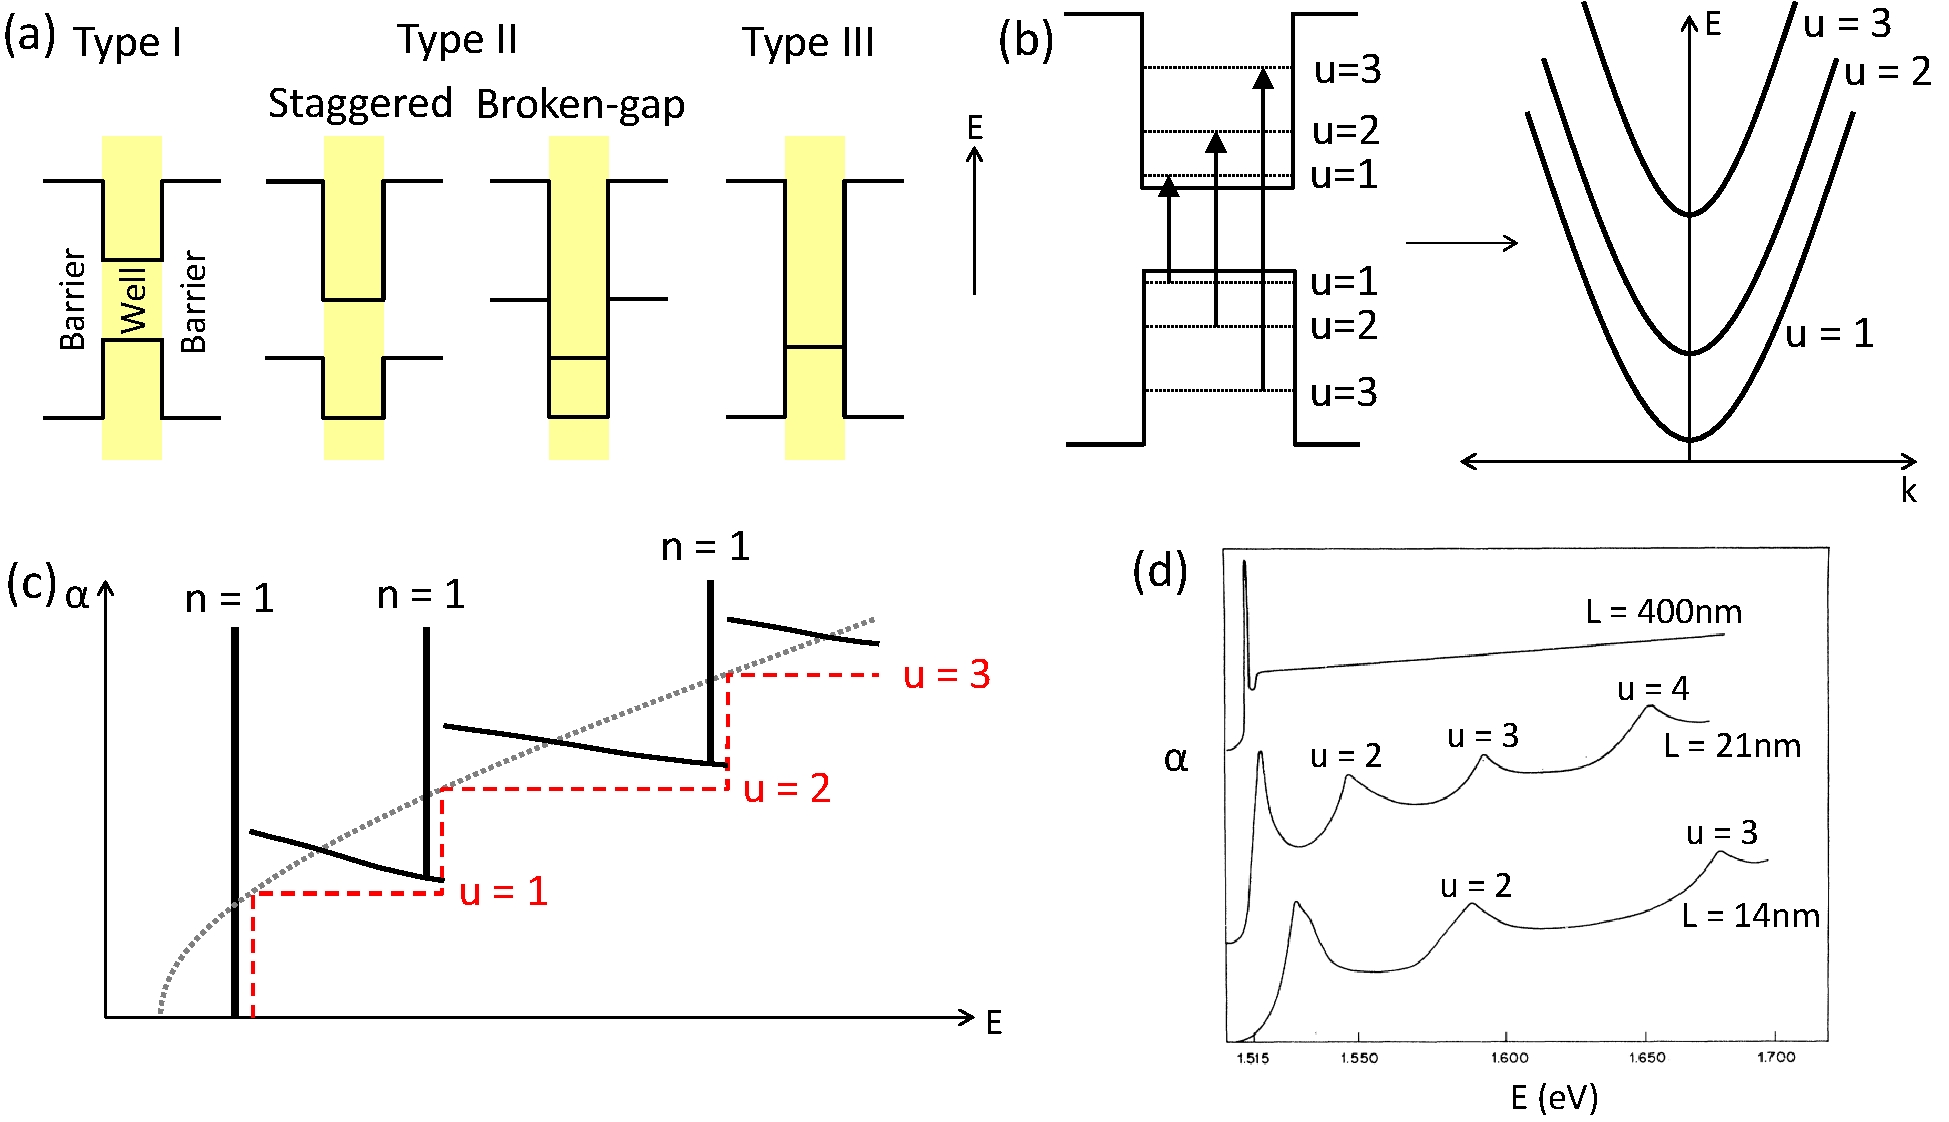
\includegraphics[width=\textwidth]{Fig2}
\caption{(a) Schematic of band structures of quantum well classifications. (b) Schematic of allowed discrete energy states inside the quantum well, and the resultant miniband structure. (c) Theoretical absorption spectrum of a 2D quantum well according to Eq.\,\ref{exabs} (black lines, not to scale). The dotted grey line shows the band edge absorption in 3D, the dashed red line the absorption in 2D, both without the Sommerfeld factor. (d) Experimental absorption spectrum of GaAs/Al$_{0.2}$Ga$_{0.2}$As quantum wells with the labelled well width $L$ at 2\,K. Only the $n=1$ excitons are observed, but the minibands $u$ are labelled. Adapted from Ref.\,\cite{Dingle1974}.}
\label{2Fig2}
\end{figure}


Exciton bands exist below each of the minibands, and in order to find $E_B$ we solve the problem of a hydrogen atom in 2D, so that
\begin{equation}
\centering
E_B =\frac{\mu e^4}{32\pi^2\epsilon^2\epsilon_0^2\hbar^2\left(n+\frac{1}{2}\right)^2} = \frac{R_H}{\left(n+\frac{1}{2}\right)^2}\frac{\mu}{\epsilon^2 m_e} .
\label{exbinding2D}
\end{equation}
Therefore the energy of the exciton bands $E_{ex}$ below the minibands can be described by
\begin{equation}
\centering
E_{ex} = \Delta E_u - E_B + \frac{\hbar^2}{2M}(k_x^2+k_y^2) ,
\label{exenergy2D}
\end{equation}
where $\Delta E_u$ describes the transition between energy levels $u$ in the CB and VB. The expected absorption spectrum of a QW structure is shown in Fig.\,\ref{2Fig2}(c), while an experimentally measured spectrum for GaAs/Al$_{0.2}$Ga$_{0.8}$As QWs are shown in Fig.\,\ref{2Fig2}(d). Note how the change in L affects the allowed $\Delta E_u$ transitions in the measured energy range, with $L=400$\,nm looking essentially like a 3D system.

We can see from Eq.\,\ref{exbinding2D} that the reduction in dimensionality leads to a factor of 4 increase in $E_B$ for the $n=1$ state, meaning exciton effects should be observable at higher temperatures in QWs. Similar $a_B$ is reduced by a factor of 2 in QWs compared to the 3D value as a result of the confinement. For this reason is it often said that excitonic effects are stronger in QWs due to increased overlap between the electron and hole wavefunctions.

\section{Properties of PbI perovskites}
Organic-inorganic metal halide semiconductors can combine the distinct properties of its organic (e.g.\ ease of processing, structural diversity, plastic mechanical properties) and inorganic (e.g.\ band structure variability, electrical mobility, thermal and mechanical stability) constituents into one composite. Two dimensional organic-inorganic perovskites self-assemble to form a multiple quantum well (MQW) structure, with alternating sheets of high band gap ($\sim6$eV) organic cations and lower band gap ($\sim3$eV) semiconducting inorganic layers \cite{Ishihara1994, Pradeesh2009b}. The wide range of organic molecules that can be incorporated into the structure enables tunability of the system \cite{Sourisseau2007}. These hybrids produce strong optical responsed, and exhibit many interesting optical properties, for example room temperature excitonic effects due to quantum and dielectric confinement \cite{Ishihara1990}, third order non-linear optical effects \cite{Xu1991a}, and biexciton effects \cite{Ishihara1992a}. Due to the self-assembled nature of the structure, such perovskites are much easier to produce than conventional inorganic QWs, and can br fabricated using a variety of techniques. Thin films of these materials can also be processed using simple techniques such as spin coating \cite{Xu1991}, making them ideal for use in optoelectronic devices.

\subsection{Structure and bonding}
Metal halide \ce{RMZ3} organic-inorganic semiconductors are based on the \ce{ABX3} perovskite crystal structure [Fig.\,\ref{2Fig3}(a)], consisting of a corner-sharing octahedra network of halogen atoms Z (most commonly I, Br or Cl), with a metal atom M in the centre of each octahedron (\ce{+2} valence metals such as Pb, Sn, Cd, Zn, Cu, Co), and organic molecules in the interstices between octahedra [Fig.\,\ref{2Fig3}(b)]. The organic molecules must fit into the interstitial space, and as a result very short molecules are used, the most common of which is \ce{CH3NH3}, which hydrogen bonds to the nearby halogen atoms. The band gaps of such semiconductors can be engineered by changing the metal and halogen composition, and recently lead halide-based semiconductors have been used as a light absorbing layer in solar cells, producing efficiencies of up to 16\%, and there is currently a drive to find lead-free alternatives for wider use \cite{Lee2012, Heo2013, Liu2013, Hao2014}. 

A change in the stoichiometric mix of organic and inorganic molecules results in the formation of lower dimension structures, for example 2D layered systems, or 1D inorganic wires \cite{Nagami1996, Fukumoto2000, Fujisawa2004, Pradeesh2010}. From here we will focus on <100> oriented 2D lead iodide (PbI) perovskites \cite{Mitzi2001}.

The structure of 2D hybrid PbI perovskites with formula \ce{(RNH3)2PbI4} are shown in Fig.\,\ref{2Fig3}(c), and consist of alternating layers of corner-sharing \ce{PbI6} octahedra and interdigitating \ce{RNH3} molecules (where R is an organic moeity). The organic molecules have larger $E_g$ (\sim6$\,eV) than the inorganic layers ($\sim3$\,eV), thus forming a type I MQW structure. The bonding in inorganic layers is primarily ionic as Pb-I distances are more comparable to the sum of ionic radii \cite{Mousdis2000}. Inorganic sheets are sandwiched between layers of organic molecules via hydrogen bonding between $\textrm{NH}_3$ groups and I atoms (see Fig.\ \ref{fig-structure}), where there are two environments for iodine atoms: bridging (shared by octahedra) or terminal (not shared by octahedra). Thus the three hydrogen atoms on $\textrm{NH}_3$ groups can adopt two hydrogen bond formations, with either two bridging iodines and one terminal iodine, or two terminal iodines and one bridging iodine. In the latter formation, the bonded iodines can either form an equilateral or right angled triangle \cite{Billing2008}. Organic molecules are usually held together by van der Waals or aromatic-aromatic interactions that can (de)stabilise the perovskite structure \cite{Mitzi2001a} and is the weak force it is possible to cleave the structure and produce mono- or few-layer regions. In this way the structure of such PbI perovskites is comparable to other layered materials such as graphene or transition-metal dichalcogenides.

\begin{figure}[ht] 
\centering    
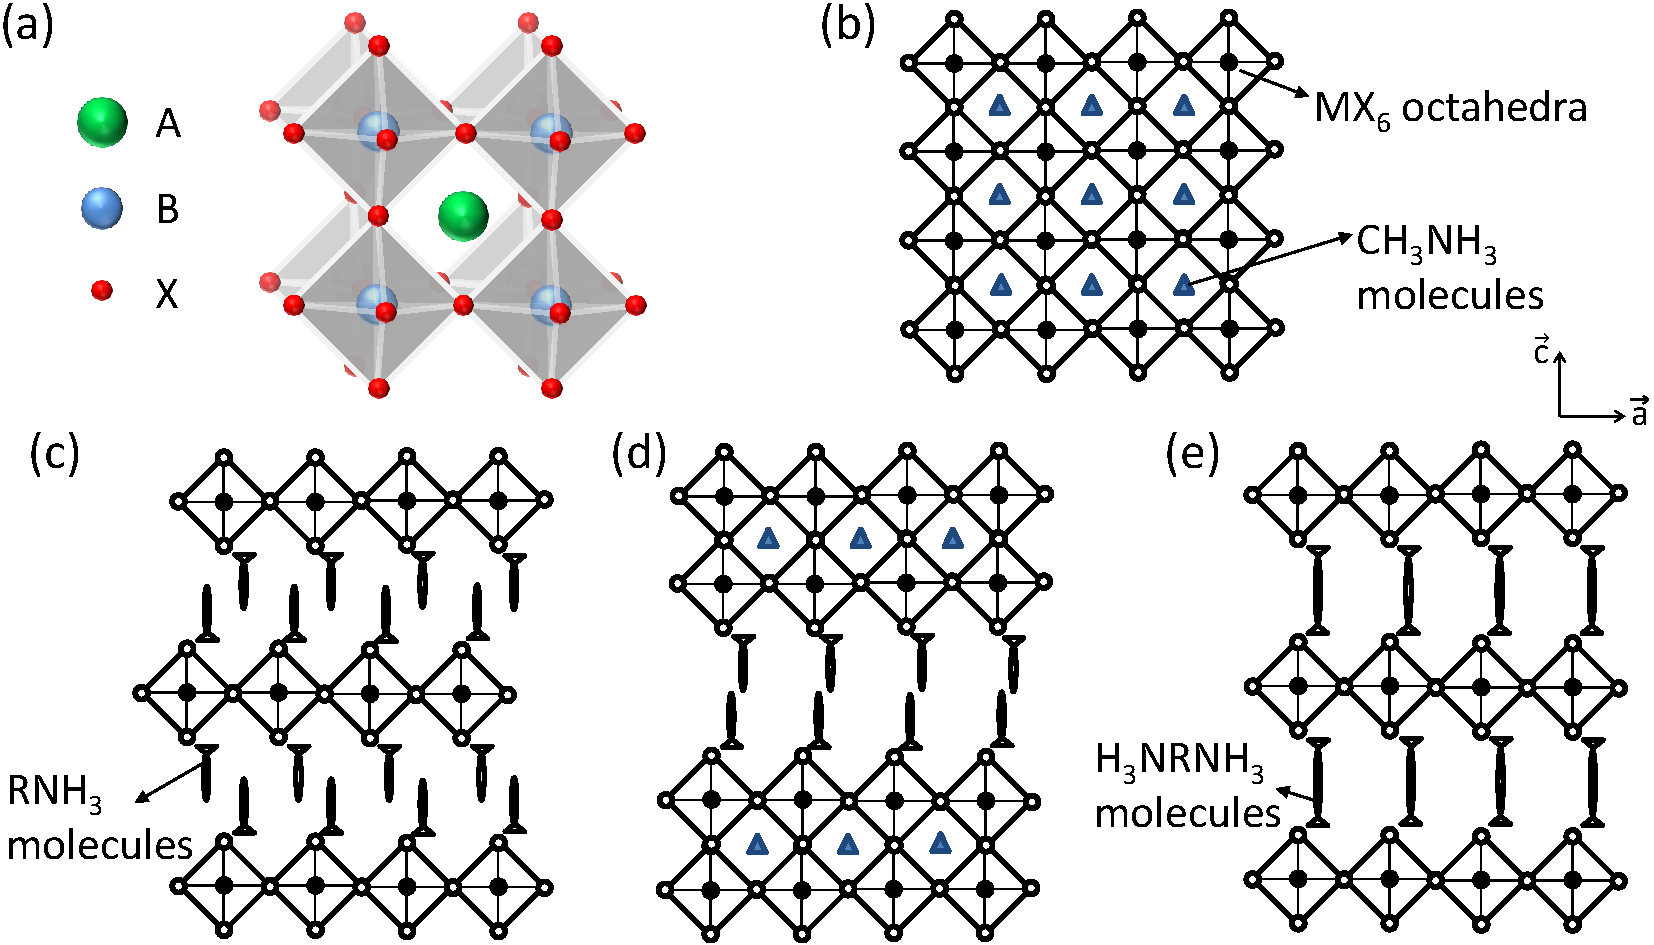
\includegraphics[width=0.8\textwidth]{Fig3}
\caption{(a) Schematic of \ce{ABX3} perovskite. Adapted from Ref.\,\cite{Perovstruc}. Structure of (b) 3D \ce{(CH3NH3)PbI3}, (c) 2D \ce{(RNH3)2PbI4}, (d) 2D multilayered \ce{(RNH3)2(CH3NH3)Pb2I7}, and (e) 2D diammonium \ce{(H3NRNH3)PbI4} viewed along the crystallographic $\vec{b}$ axis.}
\label{2Fig3}
\end{figure}

he width of the inorganic layer, defined as the width of the PbI octahedra, is typically around 6.5\AA~\cite{Ishihara1989}, whereas the organic layer width is obviously molecule dependent. There are two main orientations for consecutive inorganic layers: eclipsed, giving a monoclinic structure, or staggered, giving an orthorhombic structure \cite{Billing2006}. The orientation chosen mostly depends on the organic molecule used, and how it fits into the overall structure. Phase transitions from the orthorhombic phase to the monoclinic phase will lead to a halving of the $c$ lattice parameter due to the increased symmetry \cite{Billing2008}.

The basic 2D layered structure can be varied in a series of ways. For instance the inorganic layers can be extended to contain multiple layers of [\ce{PbI6}] octahedra [Fig.\,\ref{2Fig3}(d)], with general formula \ce{(RNH3)2(CH3NH3)}$_{n-1}\textnormal{Pb}_n\textnormal{I}_{3n+1}$ \cite{Calabrese1991}, thus varying the width of the quantum wells. Another is with the use of diammonium organic molecules, which can hydrogen bond to two consecutive inorganic layers, therefore elinating the need for van der Waals interactions between the interweaving molecules. The general formula for such systems is \ce{H3NRNH3)PbI4}, and the structure is shown in Fig.\,\ref{2Fig3}(e).

There is little limit on the organic molecule R that can be used in the structure. The cross section of the organic molecule should be small enough so that it can fit into the interlayer space between four adjacent octahedra, and must have a cross-sectional area $\lesssim 40$\,\AA$^2$  \cite{Mitzi2001a}. However their lengths are not constrained so long as the intermolecular forces are strong enough to hold the structure together. Systems with aromatic molecules tend to be better organised with more crystallinity, since such molecules allow for self-assembly using stronger aromatic-aromatic interactions \cite{Zhang2009}. Large organic R groups will also hinder self assembly and reduce crystallinity \cite{Zhang2009}. In general very simple organic molecules are used, for example those based on simple alkane chains ((\ce{Cn}$\textnormal{H}_{2n+1}$\ce{NH3)2PbI4}, C$_n$PI hereafter), ring structures (\ce{(C6H9NH3)2PbI4}, CHPI), or aromatic molecules (\ce{(C6H5C2H4NH3)2PbI4}, PAPI). However more complex organic molecules can be used, for example optically active ligands \cite{Billing2006, Teshima2003} and fullerene derivatives \cite{Kikuchi2005, Kawabata2009}. The formation of perovskite structure was particularly problematic due to the large size of the fullerene molecules, however band gap of the ligands gave rise to energy transfer between organic and inorganic layers.


\subsubsection{Phase transitions in $\textrm{C}_n$PI}
Four main phases of $\textrm{C}_n$PI perovskites have been identified: at low temperatures, $\lesssim -30^{\circ}$C (phase I), the crystal exhibits twinning so atomic positions cannot be determined. Above this, between $\sim-30$ and $15^{\circ}$C  (phase II), organic chains are ordered. At room temperature, between $\sim 15$ and $65^{\circ}$C (phase III), organic chains have become disordered, and at high temperatures, above $\moresim 65^{\circ}$C (phase IV), organic chains appear to be ``melting" \cite{Ishihara1990, Xu1991, Ishihara1989}. For $\textrm{C}_{12}$-, $\textrm{C}_{14}$-, $\textrm{C}_{16}$-, and $\textrm{C}_{18}$PI phase III is orthorhombic with staggered inorganic sheets, and phase IV is monoclinic with eclipsed inorganic sheets \cite{Billing2008}. The changes in structure are shown in Fig.\ \ref{fig-billing2008-1}. The transition between phases II and III is known as ``pre-melting", and causes dynamic rotational disorder of [$\textrm{NH}_3$] groups in $\textrm{C}_{12}$-, $\textrm{C}_{16}$-, and $\textrm{C}_{18}$PI, actually leading to a small decrease in the $c$ lattice parameter \cite{Barman2003}. Above the transition, there is a sharp increase in conformational disorder as the alkylammonium chains become tilted at different angles, leading to a large increase in $c$, and thus an increase in volume since no lateral motion occurs \cite{Barman2003}. Simulations show that after the melting transition alkyl chains are no longer all-trans, and the introduction of gauche defects leads to a shortening of the chain and an increase in its effective cross-sectional area. Conflicting demands of close packing that optimise dispersive interactions and the larger area required by conformationally disordered chains can no longer be met by a uniformly tilting arrangement, and the non-uniform tilt allows for increased space for individual chains \cite{Naik2010}. 

Changes in conformation during phase transitions also cause a spatial shift in the coupling between $\textrm{NH}_3$ groups and inorganic octahedra \cite{Pradeesh2009}. In order to accommodate the changes in alkyl chains, $\textrm{PbI}_6$ octahedra can undergo two types of structural change: they can tilt perpendicular or parallel to the inorganic sheets. During perpendicular tilting octahedra are tilted with respect to each other, whereas parallel tilting leads to an overall corrugation of inorganic layers \cite{Billing2008}. 

\begin{figure} [ht]
\centering
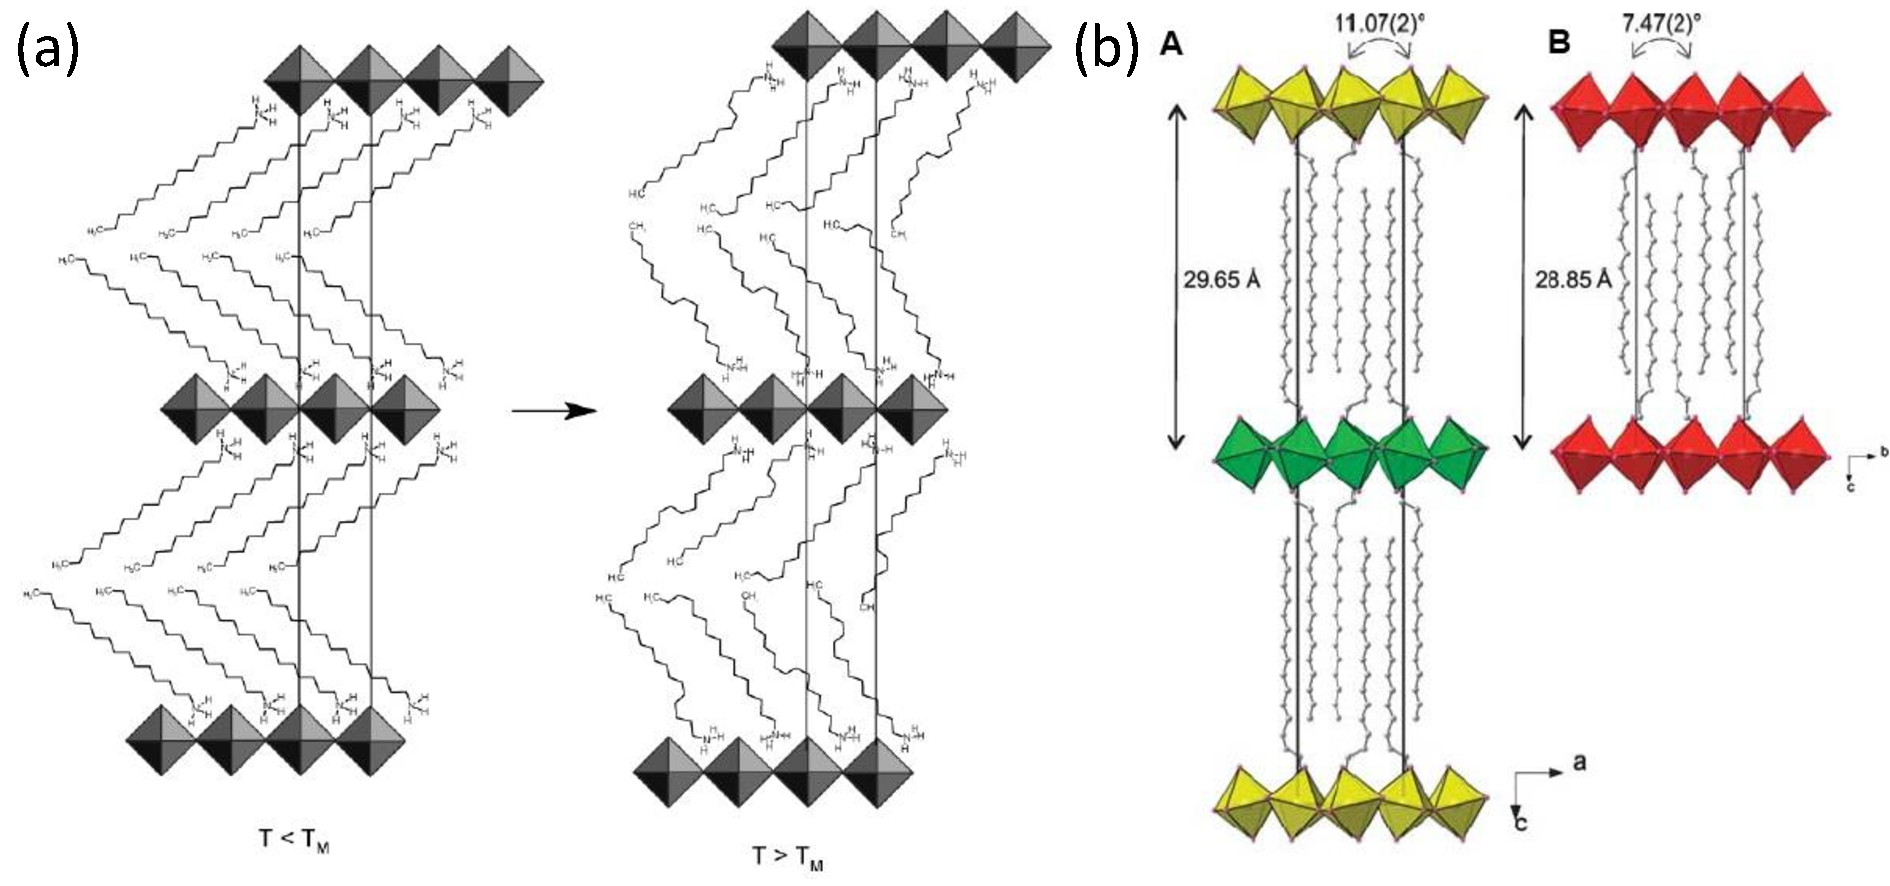
\includegraphics[width=\textwidth]{Fig4}
\caption {(a) Structure of $\textrm{C}_{n}$PI ($n$=12, 14, 16, 18) before (A) and after (B) the pre-melt transition. A is orthorhombic, and B is monoclinic so the lattice parameter $c$ is halved. (b) Schematic of the melting transition in $\textrm{C}_{10}$PI. Below the melting temperature $T_M$, the chains adopt an all-trans conformation (no gauche defects \cite{Naik2010}) with a well defined tilt angle of around $55^{\circ}$ \cite{Venkataraman2002, Venkataraman2002a}. Above $T_M$, alkylammonium chains are conformationally disordered with different tilt angles. (a) Reproduced from Ref.\ \cite{Billing2008}, (b) from \cite{Barman2003}.}
\label{2Fig4}
\end{figure}

The switching between orthorhombic and monoclinic phases does not only occur because of temperature changes. Pradeesh \textit{et al.}\ showed that the phases present in spin coated films of $\textrm{C}_{12}$PI depended on the thickness of the sample, as well as aging effects. They postulated that this was due to strain effects, where high strain in thicker samples favours the flatter orthorhombic phase. Aging effects, where a sample in the monoclinic phase gradually shifted to the orthorhombic phase, were stopped by annealing the samples or capping them with PMMA. Hysteresis was seen in the thin films during heating-cooling cycles, and the high temperature phase found to be metastable below the transition temperature as sample strain impeded the transition \cite{Pradeesh2009}.

\subsection{Fabrication and processing techniques}
\subsubsection{Silica-gel method}
An aqueous solution of Pb($\textrm{CH}_3 \textrm{COO)}_2$, $\textrm{C}_n\textrm{H}_{2n+1}\textrm{NH}_2$, $\textrm{CH}_3$COOH, and $\textrm{Na}_2\textrm{SiO}_3$ is prepared in a test tube, and becomes a gel after approximately one week. At this point an aqueous solution of KI is poured into the gel and the $\textrm{I}^-$ ions diffuse slowly into the gel to form $\textrm{C}_n$PI single crystals. About a month after the introduction of KI, platelet-like crystals form, approximated $2\times 2\times 0.1$~mm in size. However crystals for perovskites where $n$=4 or 6 cannot be produced using this method \cite{Ishihara1990}.

The silica-gel method allows multiple components to be mixed in solution on a nanometer scale, which can produce very homogeneous materials. The technique can also be used to make thin films by dissolving the raw ingredients in a suitable solvent (e.g. an alcohol) that is fast gelling and drying. The necessary condensation reaction and solvent evaporation will take place after the solution has been applied to a substrate, leaving behind a gel film. The wet film can then be heated to produce a dry film, but in order to avoid cracking the wet film should generally be less than 1~$\mu$m thick. The thin gel films are usually amorphous, but surfactants on the substrate can help with assembly, and annealed films are generally crystalline \cite{Mitzi2001b}.

\subsubsection{Solution crystal growth}
Although single crystals can be produced using the silica-gel method, it is rather time intensive. More commonly crystals of a similar or larger size can be produced from solution. Pb$\textrm{I}_2$ and the organic ammonium iodide (e.g.\ R$\textrm{NH}_3$I for $(\textrm{RNH}_3)_2\textrm{PbI}_4$, produced by reacting R$\textrm{NH}_2$ and HI) are usually mixed in stoichiometric amounts (e.g.\ \cite{Kitazawa1996, Tang2001}) in solution and left for the solvent to evaporate \cite{Ishihara1994}. After about a week single crystals form, although the rate of evaporation can be controlled to change the morphology of crystals \cite{Cheng2010}. The difficulty lies in finding solvents that will dissolve both the inorganic and organic parts of the perovskites, and examples include acetone \cite{Hong1992}, DMF \cite{Kitazawa1996}, and HI \cite{Barman2003}.

\subsubsubsection{Layered solution method}
A layered solution method can be used to create $(\textrm{C}_6\textrm{H}_5\textrm{C}_2\textrm{H}_4\textrm{NH}_3)_2\textrm{PbCl}_4$ (PAPC) at room temperature. Pb$\textrm{Cl}_2$ in concentrated aqueous HCl is placed in a tube, followed by a less dense layer of methanol, carefully placed using a syringe. Finally a stoichiometric quantity of $\textrm{C}_6\textrm{H}_5\textrm{C}_2\textrm{H}_4\textrm{NH}_2$ (relative to Pb$\textrm{Cl}_2$) is added at the top of the column as shown in Fig.\ \ref{2Fig5}, which then disperse into the methanol. As the layers slowly diffuse together, crystals of PAPC form at the interface between the Pb$\textrm{Cl}_2$/HCl and methanol layers. X-ray diffraction (XRD) studies confirm that crystals had the structure expected \cite{Mitzi1999b}.

\begin{figure}[ht]
\centering
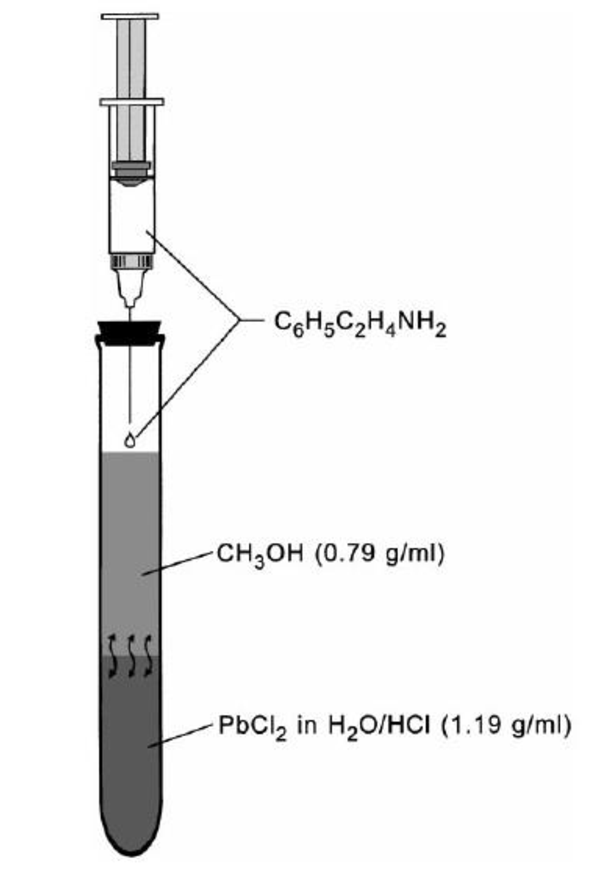
\includegraphics[width=0.35\textwidth]{Fig5}
\caption{Schematic of experimental set up used for the layered solution method of crystal growth. Crystals were formed at the Pb$\textrm{Cl}_2$/HCl and methanol interface. Densities of the pure solvents are shown in brackets. Reproduced from Ref.\ \cite{Mitzi1999b}.}
\label{2Fig5}
\end{figure}

\subsubsection {Spray pyrolysis/drying}
Spray pyrolysis produces particles when misted streams of precursor solution are introduced to a furnace. The solvent evaporates, followed by diffusion and separating out of solute, drying, precipitation, and a reaction between components in the tubular furnace reactor. Multicomponent particles can be prepared via spray pyrolysis due to microscale reactions happening inside the micro-sized droplets, and new phases with narrow size distributions and non-agglomeration can be obtained rapidly due to the high temperature and inert gas stream inside the furnace reactor \cite{Cheng2005}. 

The precursor solution used to prepare a PAPI powder consists of stoichiometric quantities of $\textrm{PBI}_2$ and $\textrm{C}_6\textrm{H}_5\textrm{C}_2\textrm{H}_4\textrm{NH}_3\cdot\textrm{HI}$ in THF.  XRD data indicate the structure is less organised than PAPI prepared by other methods, e.g.\ spin coating, and from FE-SEM images the powder particles appear to be $\sim 1 \mu$m in size. The photoluminescence (PL) spectrum of PAPI powder showed a strong exciton peak, indicating the formation of the required layered structure. However the wavelength is shifted by around 5~nm, which is probably due to distortion and a different linkage of $\textrm{PbI}_6$ octahedra \cite{Cheng2005}.

A similar technique of spray drying can be used to produce perovskite nanoparticles. The precursor solution is prepared by bubbling a flow of dry HI into a dry ethereal solution of organic amine. Drying droplets (initial mean diameter $\sim 35~\mu$m) are carried from the aerosol generator by dry air into an evaporation chamber settled in an oven heated at $250^{\circ}$C. Dried particles are collected as made and stored at room temperature. Nanoparticles created using this method are mostly spherical, but with a large size distribution ($50-500$~nm diameter; average $60\pm10$~nm). The perovskite actually crystallises at the edge of the particle while the centre is depleted, therefore larger nanoparticles are hollow. Smaller particles dry too fast for the above process to take effect, and are therefore denser. XRD data indicates the nanoparticles are crystalline, with a small red-shift of a few nm in PL exciton energy. The nanoparticles are much larger than the Bohr radius of excitons, so the shift is likely due to strain effects caused by spray drying, not quantum confinement. The nanoparticles are also fairly photo-stable, with a drop in PL intensity of around 30-50\% after illumination of 1hr \cite{audebert2009}.

\subsubsection {Langmuir-Blodgett technique}
The Langmuir-Blodgett (LB) technique uses a movable barrier to apply pressure to a monolayer of molecules at a liquid-gas interface. The applied pressure causes molecules to be close enough so that van der Waals forces can achieve close packing, thus forming a thin film (see Fig.\ \ref{2Fig6}) \cite{Mitzi2001b}. Era \textit{et al.}\ used LB to create thin films of $(\textrm{C}_{22}\textrm{H}_{45}\textrm{NH}_3)_2\textrm{PbBr}_4$. The long chain ammonium bromide ($\textrm{C}_{22}\textrm{H}_{45}\textrm{NH}_3$Br) is spread on an aqueous subphase containing Pb$\textrm{Br}_2$ and $\textrm{CH}_3\textrm{NH}_3$Br from a chloroform and DMF solution. The monolayer is then pressed to a surface pressure of 30mN$\textrm{m}^{-1}$, then deposited on hydrophobidised fused quartz substrates. Two layers of the monolayer are required to create the MQW structure needed. The just deposited film shows a strong exciton absorption peak, indicating the formation of the quantum well structure, and remain unchanged for more than 12~hours \cite{Era2000}. Fig.~\ref{2Fig6} shows the absorption spectra after multiple depositions.
\begin{figure} [h]
\centering
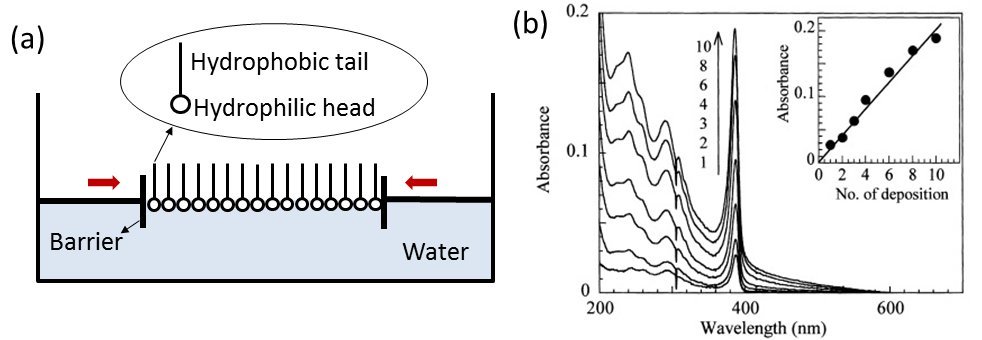
\includegraphics[width=\textwidth]{Fig6}
\caption{(a) Schematic of Langmuir-Blodgett setup, with (A) a bath containing (B) the monolayer of amphiphilic molecules at the gas-fluid interface, (C) the substrates being withdrawn from the bath, and (D) a balance that measures the surface pressure of the monolayer, generated by the movable barrier. (E) The moving barrier is controlled by a feedback device (F), which gets information from the pressure sensor and adjusts the barrier position using the (G) motor. (b)Absorption spectra of LB film obtained using the labelled number of depositions. Inset shows exciton absorbance intensity against the number of depositions, and it can be seen that the absorbance is increased as the films become thicker with an increasing number of depositions. (a) reproduced from Ref.\ \cite{Mitzi2001b}, and (b) reproduced from Ref.~\cite{Era2000}.}
\label{2Fig6}
\end{figure}

\subsubsection{Intercalation}
Although there has been no direct investigation, it is believed that the driving forces for self assembly in PbI perovskites include a preference for the inorganic octahedra network, the hydrogen bonding between $\textrm{NH}_3$ groups and inorganic sheets, and the construction of interdigitated organic groups by van der Waals/aromatic-aromatic bonds \cite{Cheng2010}. Thus perovskite films can be formed by the intercalation of organic molecules into the inorganic framework. Pb$\textrm{I}_2$ films are deposited onto substrates by vacuum deposition or spin coating, and a solution of organic ammonium iodide prepared. The Pb$\textrm{I}_2$ covered substrates are dipped in the iodide solution, then the iodide solution solvent to remove excess organic salts, and finally pumped in the loading dock of the drybox used in order to remove all remaining solvents. The resulting films have the same properties as films created using other methods \cite{Liang1998}. The film thickness is controlled by the initial Pb$\textrm{I}_2$ film thickness, and in the case of $\textrm{(C}_6\textrm{H}_9\textrm{C}_2\textrm{H}_4\textrm{NH}_3)_2\textrm{PbI}_4$ (CHPI) only 10s in the iodide solution was needed in order to complete intercalation \cite{Pradeesh2009a}.

A similar dipping method has been used to make thin films of $\textrm{C}_{12}'$PI. $\textrm{INH}_3(\textrm{CH}_2)_{12}\textrm{NH}_3\textrm{I}$ is dissolved in dioxane, then diluted with water to create a 5mM solution. A $\textrm{PbI}_2$/dry oxane solution is also created, and quartz substrates cleaned in a solution of $\textrm{H}_2\textrm{SO}_4$ and $\textrm{H}_2\textrm{O}_2$, then rinsed with distilled water and methanol. The hydrophillic quartz substrates are dipped in the iodide solution for 20mins, then immersed in a dioxane/water solution for 5mins to remove excess organic salts. Substrates are then dipped in the $\textrm{PbI}_2$ solution for 15mins, and finally washed with dioxane. The procedure can be repeated as needed in order to achieve multilayers of self assembled quantum wells and control the films thickness \cite{Matsui2002}.

Gaseous intercalation has also been demonstrated by Era \textit{et al.}. A 20~nm thick film of Pb$\textrm{I}_2$ is vacuum deposited on a quartz substrate, then exposed to vaporised organic ammonium iodide ($\textrm{C}_6\textrm{H}_5\textrm{C}_2\textrm{H}_4\textrm{NH}_3\textrm{I}$). Both XRD and absorption confirm the formation of PAPI, although in XRD signatures of Pb$\textrm{I}_2$ were still seen \cite{Era1998}.

Recently in-situ measurements on liquid-phase intercalation has shown that intercalation occurs from the top surface of the \ce{PbI2} film, and proceeds in a direction perpendicular to the inorganic layers. Organic molecules attaches to the top surface of the \ce{PbI2} layer has terminal groups, therefore transforming the face-sharing PbI octahedra into a corner-sharing network, opening interstices for organic molecules to diffuse through and interact with the bottom surface of the same layer, thus converting the \ce{PbI2} layer into full 2D monolayer. Further diffusion continues intercalation for layers further from the interface [Fig.\,\ref{2Fig7}]. This process requires a non-polar solvent that will not compete with the hydrogen bonding between the inorganic and organic constituents, while steric hindrance between molecules also plays a role in the dynamics, thereby producing an optimum organic iodide concentration for the intercalation solution \cite{Ahmad2014}.

\begin{figure} [ht]
\centering
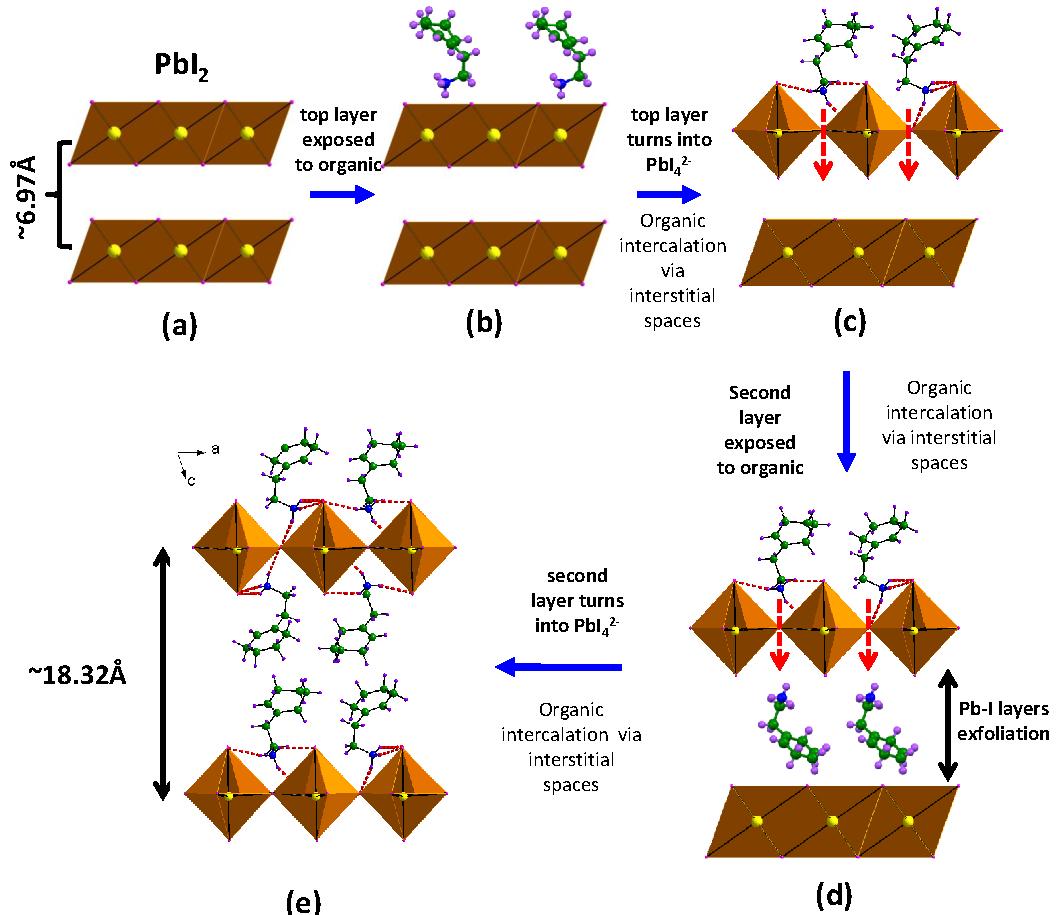
\includegraphics[width=\textwidth]{Fig7}
\caption{Schematic of liquid-phase intercalation dynamics of organic ammonium iodide molecules into \ce{PbI2} film. Reproduced from Ref.\,\cite{Ahmad2014}.}
\label{2Fig7}
\end{figure}

\subsubsection{Dual-source vacuum deposition}
PAPI films were also created using a dual-source vacuum deposition method, where both Pb$\textrm{I}_2$ and $\textrm{(C}_6\textrm{H}_9\textrm{C}_2\textrm{H}_4\textrm{NH}_3)\textrm{I}$ were vacuum deposited simultaneously on a quartz substrate with rates of 7.1 and 21ng~$\textrm{cm}^2\textrm{s}^{-1}$ respectively. The created film showed the same sharp exciton absorbance peak as films created by other methods, however the XRD pattern of the film showed no peaks at high $\theta$, so the films were disordered and possibly defective. The growth of the layered perovskite structure appears to occur in the solid phase on the substrate \cite{Era1997}. In addition the organic ammonium halide may dissociate into an amine and HI, so care needs to be taken with choice of evaporation rates, or else films can be multiphasic, disordered or defective \cite{Mitzi1999}.
\begin{figure}[ht]
\centering
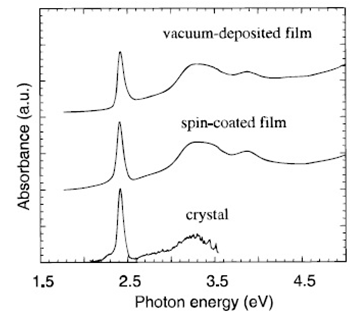
\includegraphics[width=0.8\textwidth]{Fig8}
\caption{(a) Schematic of dual-source vacuum deposition process. Deposition rates of the two sources needs to be controlled carefully in order to create a non-defective film. (b) Comparison of absorbance spectra of a vacuum deposited film, a spin coated film, and a single crystal sample of PAPI, where there appears to be very little difference between the three different methods. Reproduced from Ref.\ \cite{Era1997}.}
\label{2Fig8}
\end{figure}

\subsubsection{Single source thermal ablation}
Single source thermal ablation involves the vaporisation of an initial material onto a substrate in order to form a film (see Fig.\ \ref{fig-chondrousdis2000-2}). The initial material can be placed on the tantalum heater as a powder (insoluble powders ideally as a suspension for better thermal and physical contact with the heater, and more even dispersion), crystal, or a concentrated solution that has been allowed to dry. The chamber is then pumped to vacuum, and a current passed through the heater. The starting material is vaporised from the heater surface and the perovskite is reassembled on substrates. The important control variable is the rate at which the heater reaches its final temperature, as a low rate may lead to multiphasic or defective films. Substrates can undergo multiple ablations, and the amount of initial material can also be used to control film thickness \cite{Mitzi1999}. AETHPI (AETH = $\textrm{C}_{18}\textrm{H}_{28}\textrm{N}_2\textrm{S}_2$) films are created using this method. Luminescence spectra show that as-formed films had only traces of a small exciton peak, so there is probably some short range order, but the MQW structure is not fully formed. Sharp exciton peaks are seen after the film is annealed, and the peak increased in intensity with annealing time as grain sizes increase. The Stokes shift also decrease with annealing time, showing an improvement in quantum well quality \cite{Chondroudis2000}.

\begin{figure} [ht]
\centering
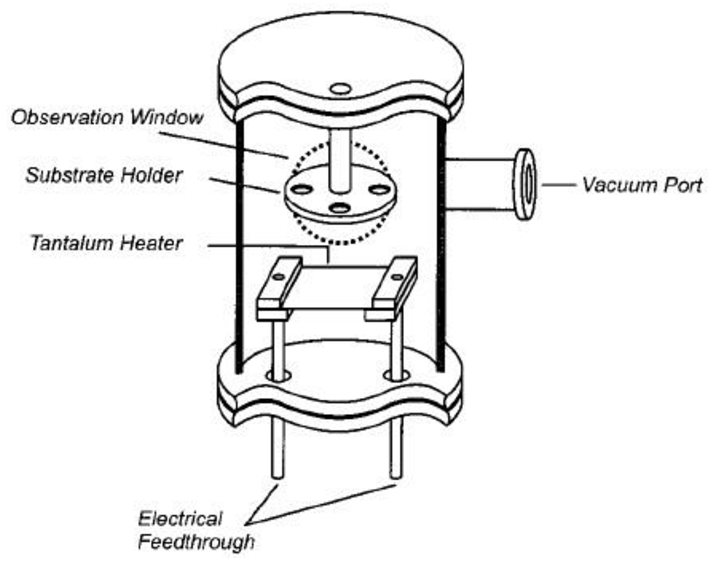
\includegraphics[width=0.5\textwidth]{Fig9}
\caption{Cross section of single source thermal ablation apparatus. The starting material is placed on the tantalum heater, then as a charge is passed through the solid sublimates and forms a thin film on the substrate above. Reproduced from Ref.\ \cite{Chondroudis2000}.}
\label{2Fig9}
\end{figure}

\subsubsection{Spin coating}
Thin films can easily be produced by spin coating a solution of PbI perovskites on a substrate (suitable solvents include DMF \cite{Kikuchi2005}, THF \cite{Kataoka1994}, and acetonitrile \cite{Prakash2009}). Drops of solution are added to spinning substrates, and as the solvent evaporates a polycrystalline film is left behind. The films produced have the same optical or electronic properties as single crystals, and the crystallographic $c$ axis perpendicular to the surface of the films \cite{Kataoka1993}. The films are generally smooth with a roughness of $\sim$1-2nm, although the solvent, substrate, perovskite solution concentration, substrate temperature, and spin speed may all affect the thickness and morphology of films. Pre-treating substrates may also improve wetting properties and affect film morphology \cite{Mitzi2001b}. In thicker films, strain and uneven crystal planes lead to stacking imperfections, which may give quantum wells of differing widths. The organic molecules may also become misaligned, and inorganic layers distorted. All these effects lead to a decrease in the intensity of exciton absorption/luminescence \cite{Prakash2009}.

PbI perovskite samples tend to degrade over time due to moisture in the air, so a PMMA matrix doped with nanocrystalline PAPI can be created in order to suppress degradation \cite{Kitazawa1998}. PPMA, Pb$\textrm{I}_2$, and $\textrm{(C}_6\textrm{H}_9\textrm{C}_2\textrm{H}_4\textrm{NH}_3)\textrm{I}$ are dissolved in DMF then spin coated onto a glass substrate, and the resulting film annealed (thickness $\approx$200nm). It can be determined through XRD that the $c$ axis in PAPI crystals are perpendicular to the surface of the film. A strong exciton absorption at 2.4eV is seen as expected, as well as a step-like feature at 2.7eV due to interband transitions (see Fig.\ \ref{fig-kitazawa1998-1}). After the PMMA doped sample is left in a humidity controlled box for two months, the spectrum appeared unchanged, but the PAPI film is degraded and no exciton peak can be seen (see Fig.\ \ref{fig-kitazawa1998-2}).  The binding energy of excitons in PMMA doped films is around 300\,meV, larger than in pure PAPI samples (around 250meV) due to dielectric confinement of PMMA. 

Adjusting the temperature and duration of annealing changes the size of the nanocrystals, but the absorption energy is not affected by the size of the crystals. On the other hand, annealing conditions do change the magnitude of the exciton absorption. At a temperature of $100^{\circ}$C, an increase in annealing time (up to 2\,hours) increases the absorption intensity as the nanocrystals become larger, although the relative absorption is not changed much [Fig.\,\ref{2Fig10}(a)]. However at $125^{\circ}$C an increase in annealing time actually reduces absorption (both absolute and relative) as PAPI crystals decompose and Pb$\textrm{I}_2$ signatures are seen in the spectra. Upon annealing for longer times, even at $100^{\circ}$C the relative absorption decreases, presumably also due to decomposition \cite{Kitazawa2002}. As seen in Figs. \ref{2Fig10}(c,d) , both annealed films are more thermally and photo-stable than pure PAPI films. Oxygen($1s$) signatures are seen in the photoelectron spectrum of photo-irradiated PAPI films, so photo-induced oxidation is a likely mechanism for photo-degradation \cite{Kitazawa2002}.

\begin{figure}
\centering
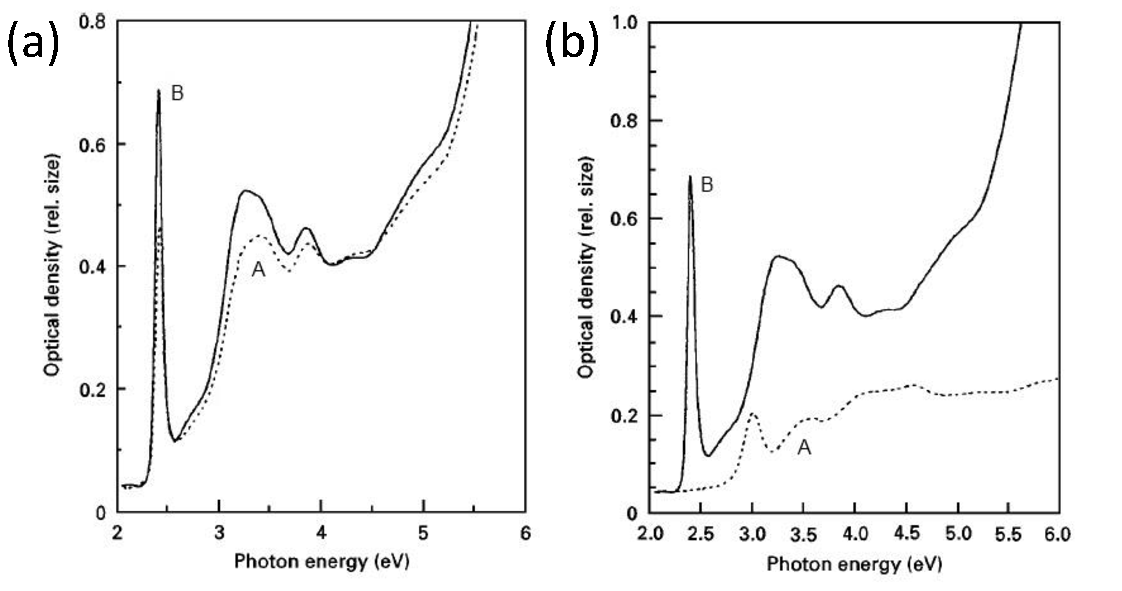
\includegraphics[width=0.8\textwidth]{Fig10}
\caption{ (a) Absorption spectra of A) PAPI film spin coated using acetonitrile solution (dotted line), and B) PAPI doped PMMA annealed at $125^{\circ}$C for 10 minutes (solid line). The spectrum for both films have the same features, although the exciton absorption intensity of A is lower. (b) Absorption spectra of above films after being in a humidity controlled box for two months. Note the exciton peak has disappeared in A as the PAPI film degraded. (c) Changes in relatively exciton absorption intensity ($I/I_0$) as function of annealing time at different annealing temperatures. (d) Changes in relative exciton absorption intensity as function of photo-irradiation time. In both (c) and (d) the doped PMMA sample at $125^{\circ}$C decomposes with annealing time, although it still absorbs more than pure PMMA film. (a) and (b) reproduced from Ref.\cite{Kitazawa1998}, (c) and (d) from \cite{Kitazawa2002}.}
\label{2Fig10}
\end{figure}

\subsubsection{Patterning}
Patterned PAPI films have been produced using a micromoulding in capillaries method (MIMIC). Moulds are created by casting PDMS on silicon master moulds, then peeling away the PDMS layer. In order to make patterned films, PDMS moulds are placed in conformal contact with pre-cleaned silicon substrates so the channels of the mould formed capillaries with the substrate. A solution of PAPI dissolved in DMF is dropped on one end, and the channels are spontaneously filled by capillary force [Fig.\,\ref{2Fig11}(a)]. The mould and solution are then cured for 2hrs at $65^{\circ}$ to evaporate the solvent. In general the film stripes in Fig.\ \ref{2Fig11}(b) are defect free, however some edge defects are seen in C (channel width 0.8~$\mu$m) since the channels are more difficult to fill when the width decreases. The width of film stripes also tend to be a little smaller than the width of mould channels, and a shrinkage of around 25\% was seen after evaporation of solvents.  The patterned films have same the optical properties as unpatterened films \cite{Cheng2003}.
\begin{figure} [ht]
\centering
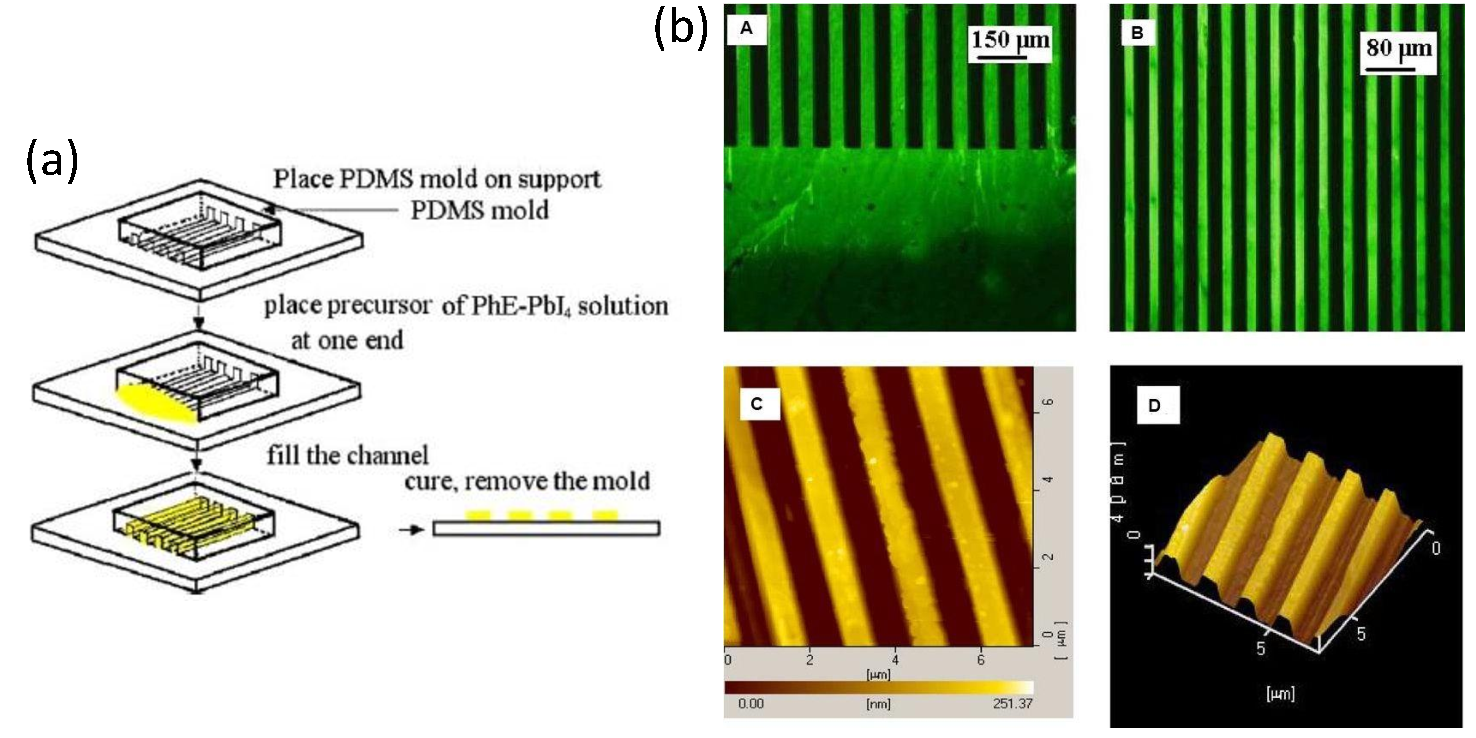
\includegraphics[width=\textwidth]{Fig11}
\caption{(a) Schematic of MIMIC process for pattering PAPI films. (b) Fluorescent optical micrographs (A,B) and AFM images (C: planar, D: stereo) of patterned PAPI films. In all cases the black stripes represent bare substrate without PAPI. Film stripes widths are A) 50~$\mu$m wide, B) 15~$\mu$m, C) and D) 0.8~$\mu$m. Note in A an unpatterned film created from left solution that did not flow into the channels. In general film stripes are defect free, however in C some edge defects are seen due to the small channel width. D shows that film stripes are organised together like trapeziform ridges. Reproduced from Ref.\ \cite{Cheng2003}.}
\label{2Fig11}
\end{figure}



\subsection{Electronic structure}

Umebayashi \textit{et al.}\ calculated the electronic structure of $\textrm{C}_{4}$PI and its 3D extension $\textrm{CH}_3\textrm{NH}_3\textrm{PbI}_3$ using linear combination of atomic orbitals (LCAO) within density functional theory (DFT) \cite{Umebayashi2003}; the calculated band structures are shown in Fig.\ \ref{2Fig12}(a). As expected, the 2D compound has a higher band gap and narrower bandwidths due to a decrease in dimensionality. The 2D band structure also has flatter dispersions at the top of the valence band (TVB) and the bottom of the conduction band (BCB), leading to a larger effective mass of carriers, and thus larger binding energy for excitons. 

Fig.\ \ref{2Fig12} also shows the bonding diagrams for a single $[\textrm{PbI}_6]^{4-}$ octahedron, as well as the 3D and 2D compounds above. In the 2D crystal the TVB consists of Pb($6s$) and I($5p$) $\sigma$-antibonding orbitals, whereas the BCB consists of Pb($6p$) and I($5s$) $\sigma$-antibonding orbitals and Pb($6p$) and I($5p$) $\pi$-antibonding orbitals (not labelled on figure). The crystal field also lifts the degeneracy between different iodine atoms, so the conduction band with bridging iodine atoms ($\textrm{I}_1$) is wider than that with terminal iodine atoms ($\textrm{I}_2$). In Ref.\ \cite{Matsuishi2004} the BCB was labelled non-bonding from first principles pseudopotential total-energy calculations with the local density approximation, although it still consisted of Pb($6p$) and I($5p$) orbitals.
\begin{figure}[h]
\centering
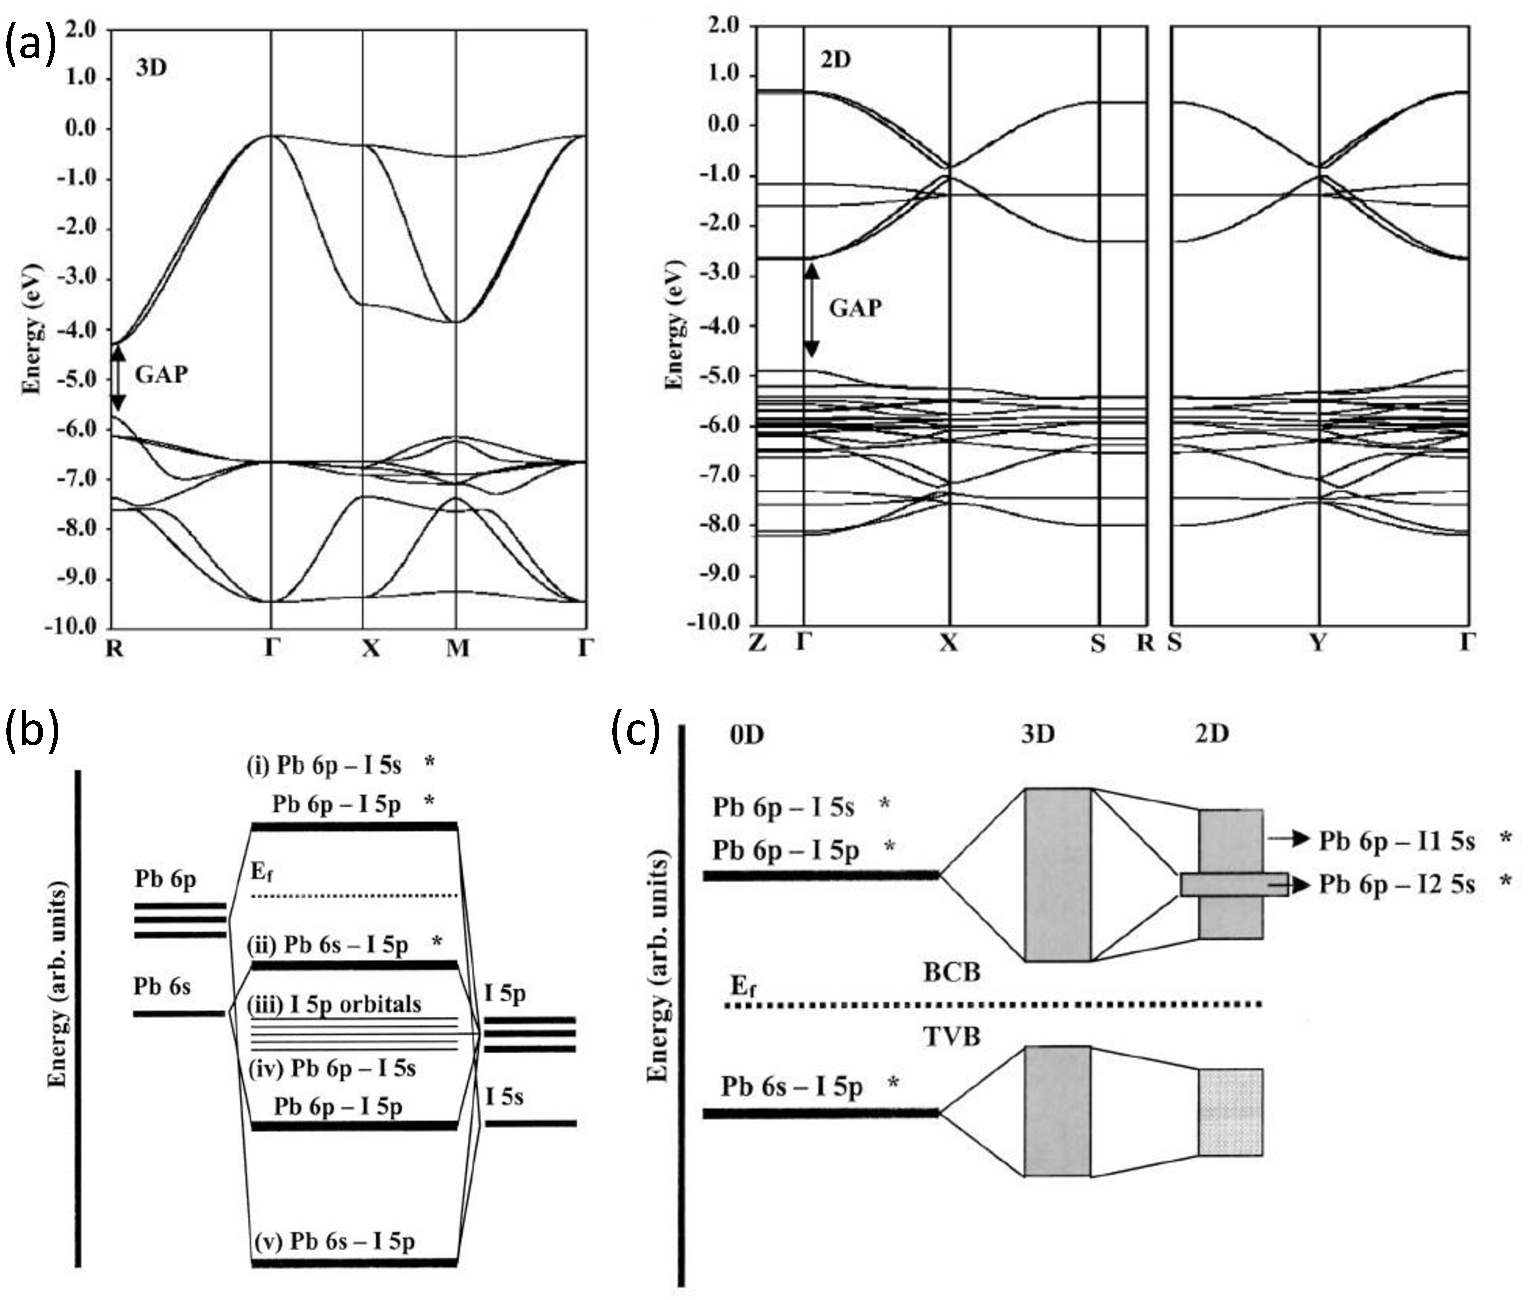
\includegraphics[width=\textwidth]{Fig12}
\caption{(a) Calculated band structures of $\textrm{CH}_3\textrm{NH}_3\textrm{PbI}_3$ (3D) and $\textrm{C}_{4}$PI (2D) along high symmetry lines in the first Brillouin zone. The band gap is labelled. Bonding diagrams of (b) individual $[\textrm{PbI}_6]^{4-}$ octahedra, and (c) extension to $\textrm{CH}_3\textrm{NH}_3\textrm{PbI}_3$ and $\textrm{C}_{4}$PI. The bottom of the conduction band (BCB), top of the valence band (TVB), and Fermi energy level ($\textrm{E}_f$) are labelled. Reproduced from Ref.\ \cite{Umebayashi2003}.}
\label{2Fig12}
\end{figure}



\subsection{Optical properties}
\subsubsection{Excitons}
Excitons are formed due to transitions between the TVB and BCB in the inorganic layers of PbI perovskites. Excitons in $\textrm{C}_{10}$PI have an energy of around 2.4~eV above 275K, and the value changes to around 2.55eV at below 268K due to a phase transition of the alkylammonium molecules [Fig.\ \ref{2Fig13}]. The binding energy $E_b$ was calculated from the difference between the exciton peak and the step-like structure (interband transitions) in absorption spectra, and a large value of 320$\pm$10meV explains the presence of excitons even at room temperature \cite{Ishihara1990}. The exciton also has a large oscillator strength of around 0.7$\pm$0.1 \cite{Ishihara1990}. The above values were for the lowest energy ($n=1$) free exciton, but bound excitons are also seen, for example in Fig.\ \ref{2Fig13}(b) the peak at 2.55~eV  is assigned to the lowest free exciton in the inorganic layers, whereas the peak at 2.53~eV decreases in intensity with temperature, and is thus assigned to a shallow bound exciton. The peaks seen at low temperature at 2.45\,eV is sample dependent, and thus assigned to deeply impurity-bound excitons. Peaks at lower energies were sample dependent, and assigned to excitons deeply bound to impurities \cite{Ishihara1990}. As seen from Fig.\ \ref{2Fig13}(c) the Stokes shift for $\textrm{C}_{10}$PI is small (less than 5~eV), and this is generally true for PbI-based perovskites (e.g. for $\textrm{C}_{12}$PI in Ref.\cite{Pradeesh2009}). In Ref.s \cite{Ishihara1990, Ishihara1989}, both longitudinal and transverse exciton-polaritons were observed in reflection spectra of $\textrm{C}_{10}$PI at 1.6~K, with a splitting of around 60meV \cite{Ishihara1990}. The exciton radiative lifetime was found to be $\approx 7$\,ps at 8\,K \cite{Kondo1998a}.

\begin{figure}[ht]
\centering
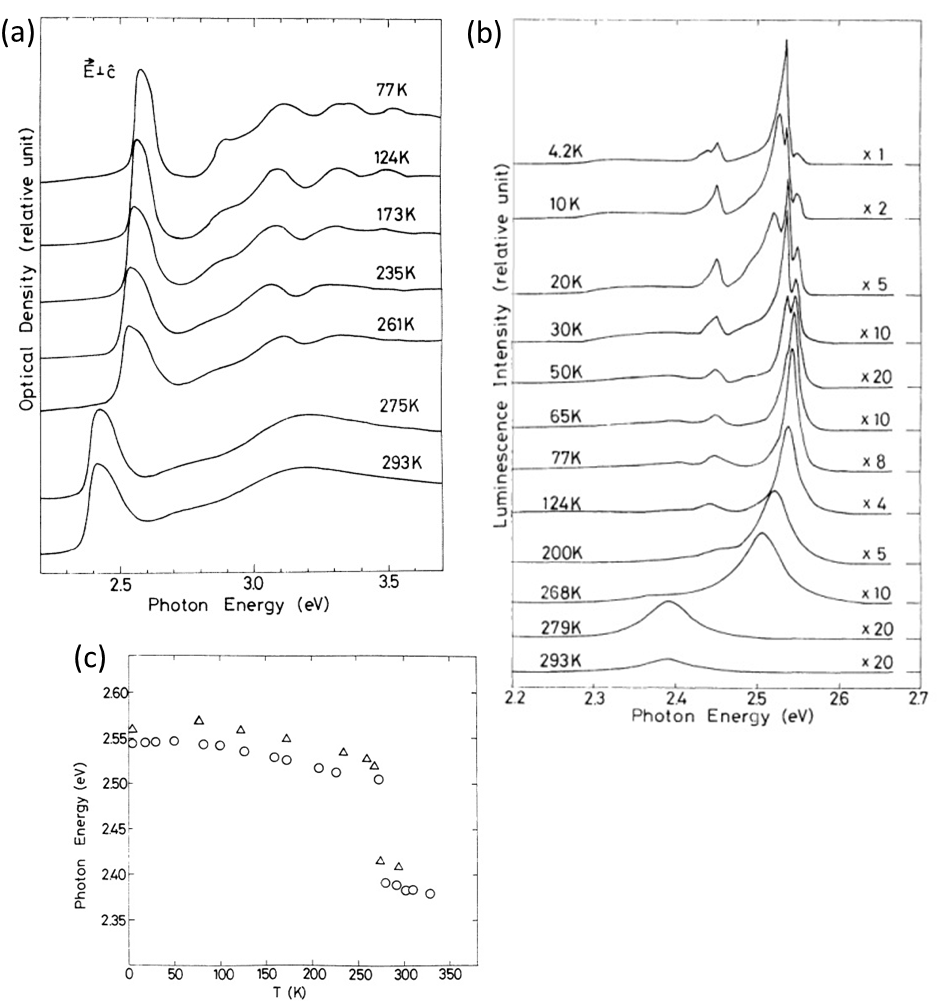
\includegraphics[width=\textwidth]{Fig13}
\caption{(a) Optical density of $\textrm{C}_{10}$PI crystal at labelled temperatures. The peak furthest left is assigned to the lowest energy free exciton, and the step-like feature next to it (seen most clearly at 77~K) is due to interband transitions. Thus the binding energy has been calculated to be 320meV. (b) Photoluminescence spectra spectra of $\textrm{C}_{10}$PI. For assignment of peaks see main text. (c) Energies of absorption ($\triangle$) and photoluminescence ($\circ$) peaks as a function of temperature, showing small Stokes shifts of around 5meV. Figures reproduced from Ref.\ \cite{Ishihara1990}.}
\label{2Fig13}
\end{figure}

Polarisation-dependent excitons were seen in the absorption spectra of $\textrm{C}_6'$PI, as calculated from Kramers-Kronig analysis of polarisation-dependent reflectivity spectra [Fig.~\ref{2Fig14}]. When the incoming light is polarised parallel to the crystallographic $b$ axis, the lowest exciton polarised parallel to $b$ is at 2.5272~eV. Two shoulders seen at 2.566 and 2.718~eV (indicated by small arrows) are due to vibronic bands. The very small peak at 2.819~eV is attributed to n=2 excitons, as determined using exciton activation energies calculated from PL spectra. Light polarised parallel to $c$ can generate excitons polarised to both the $\vec{a}$ $\textrm{and}$ $\vec{c}$ axes since the crystal is monoclinic, so the narrow peak at 2.559~eV is due to excitons polarised parallel to $\vec{c}$. As the $\vec{a}$ and $\vec{b}$ directions are very nearly isotropic, the peak at 2.5272~eV, also seen in Fig.~\ref{2Fig14}(a), is attributed to excitons polarised parallel to $\vec{a}$. However the peak due to the exciton parallel to $\vec{c}$ only appears at very low temperatures, as the peak width normally makes the two exciton peaks indistinguishable. The $n=2$ peak is seen at the same position as in Fig.~\ref{2Fig14}(a). The binding energy for the material is calculated to be 330meV, and the Bohr radius 8.2\AA \cite{Goto2001}.

\begin{figure} [ht]
\centering
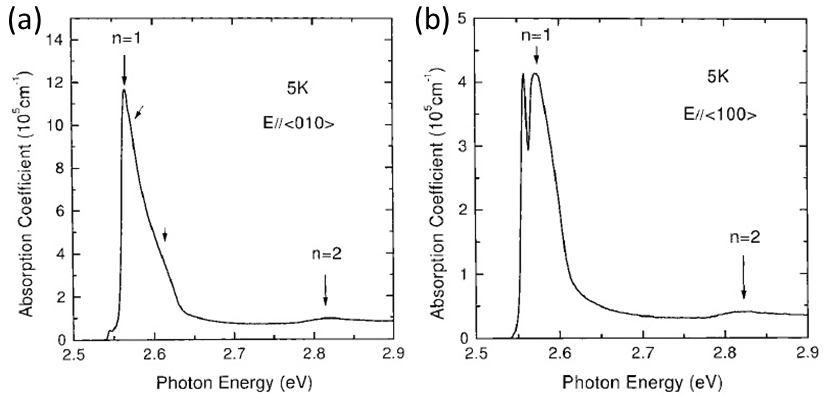
\includegraphics[width=\textwidth]{Fig14}
\caption{Absorbance spectra for {\bf E} // crystallographic (a) $\vec{b}$, and (b) $\vec{c}$ axes for \ce{C6PI}, calculated using Kramers-Kronig relations from reflection spectra. In (a) the $n=1$ peak is due to excitons polarised parallel to $\vec{b}$, and the shoulders are seen due to vibronic bands. In (b) the sharp $n=1$ peak is attributed to excitons polarised parallel to $\vec{c}$, whereas the broad $n=1$ peak is due to excitons polarised parallel to $\vec{a}$. Reproduced from Ref.\ \cite{Goto2001}.}
\label{2Fig14}
\end{figure}

There has been some discussion regarding whether the excitons are Wannier- or Frenkel-like in nature. Xu \textit{et al.} used magneto-optical measurements on polycrystalline $\textrm{C}_{10}$PI thin films and found that exciton peaks were not shifted when a magnetic field $B$ was applied in the plane of the film, but when the field was applied perpendicular to the plane of the film the energy of the exciton changed according to
\begin{equation}
E = E_0 \pm \frac{1}{2} g_{\bot} \mu_{B} B + c_0 B^2~,
\label{mag-shift}
\end{equation} 
where $E$ is the energy of the exciton, $E_0$ is the energy of the exciton at zero field, $g_{\bot}$ is the Land\'{e} $g$ factor perpendicular to the plane of the film, $\mu_B$ is the Bohr magneton, and $c_0$ is the diamagnetic constant. The energy shift depends on the polarisation of the magnetic field (plus sign for $\sigma^+$ and minus sign for $\sigma^-$), and both $g_{\bot}$ and $c_0$ depend on exciton wavefunction. Calculated value showed $g_{\bot}$ were $\sim1$, and $c_0$ $\sim 10^{-7}$~eV/$\textrm{T}^2$. From the magneto-absorption measurements the Bohr radius $a_0$ of $\textrm{C}_{10}$PI was estimated to be 12\AA. The peak shifts indicate $\textrm{C}_{10}$PI excitons are Wannier-like, since Frenkel excitons would have no extended motion and thus show no energy shift at all. However as the size of each $\textrm{[PbI}_6]$ octahedron is around 6\AA~\cite{Ishihara1990}, so excitonic motion only extend over a few octahedra \cite{Xu1991b}. Further magneto-optical measurements revealed a small anisotropy in the 2D $a-b$ plane, as well as evidence of strong interaction between the exciton and phonon modes (phonon sidebands), suggesting a small extension of the internal wavefunction of the exciton \cite{Hirasawa1993}.

$\textrm{C}_{6}$PI crystals were used in magneto-optical measurements, and the samples were of good enough quality that a single peak in Ishihara's measurements could be resolved into an exciton peak and its phonon sidebands. The calculated $g_{\bot}$ and $c_0$ values were similar to those in $\textrm{C}_{10}$PI, however the authors believed that as the exciton Bohr radius is on the order of Pb-Pb distances in the crystal, the exciton may be better described by the Frenkel model (exciton wavefunctions made of $s$ and $p$ orbitals of the $\textrm{Pb}^{2+}$ cation, and involve transitions from the $(ns)^2$ to $(ns)(np)$ molecular orbitals). The orbital wavefunctions of $\textrm{Pb}^{2+}$ were then used to calculate $g_{\bot}$ and $c_0$, and the results agreed well with experiment \cite{Kataoka1993}. On the other hand Tanaka \textit{et al.}\ used electroabsorption and two-photon absorption studies and showed that excitons in thin film $\textrm{C}_{6}$PI samples were Wannier-like in nature, with 1s, 2s, 2p, and 3p energies at 2.34, 2.60, 2,61, and 2,64~eV respectively. The Wannier excitons exhibited strong 2D behaviour, with a large binding energy of the 1s exciton (310meV) \cite{Tanaka2002}.

The band gap of the material can be engineered by altering the halogen and metal atoms in the perovskite structure, thus tuning the exciton energy. The exciton energy ranges from 2.5\,eV for PbI perovskites, to 3.1\,eV for PbBr and 2.6\,eV for PbCl. Indeed mixed-halide perovskites of the form \ce{(RNH3)2Pb}$\textnormal{A}_x\textnormal{B}_{1-x}$ allows to further variation within this range \cite{Kitazawa1996, Kitazawa1997}. It has been shown that the while the change in absorption wavelength generally varies linearly with the halogen concentration $x$ as the process is averaged over excitons at all possible sites, the excitons formed then preferentially diffuse to lower energy halogen atomic sites, thus emission wavelength does not show the same linear variation with $x$ \cite{Ahmad2013}.


\subsubsection{Biexcitons and triexcitons}
An increase in excitation power can lead to the formation of bi- or tri-exciton complexes, where two or three free excitons are bound together. On the other hand, induced photo-carriers screen Coulomb interactions and make complexes less stable, so electron-hole plasmas usually form before triexcitons. In order to see triexcitons there needs to be a strong Coulomb interaction between carriers to withstand screening, and a low dimensionality also helps as screening by carriers only has a limited effect \cite{Shimizu2006a}. The radiative decay of a biexciton to a transverse exciton has been observed in $\textrm{C}_{10}$PI, with biexciton binding energy of $\approx$ 50meV \cite{Ishihara1992}. By creating a waveguide configuration (200nm $\textrm{C}_{6}$PI film spin coated on Ti-containing Si$\textrm{O}_2$ with Al-mirrors formed on the optically flat output faces of the substrate) with transverse pumping, biexciton lasing was observed in $\textrm{C}_6$PI. The lasing threshold is 20~kW/$\textrm{cm}^2$ at 16~K and increases sharply with temperature. Fig.\ref{2Fig15}(b) shows emission spectra above and below the lasing threshold: a broad biexciton band is seen below the threshold, but a sharp peak at 2.281V is seen above the threshold. The biexciton band is probably isotropic as the emission was not polarised \cite{Kondo1998}.

\begin{figure}[h!]
\centering
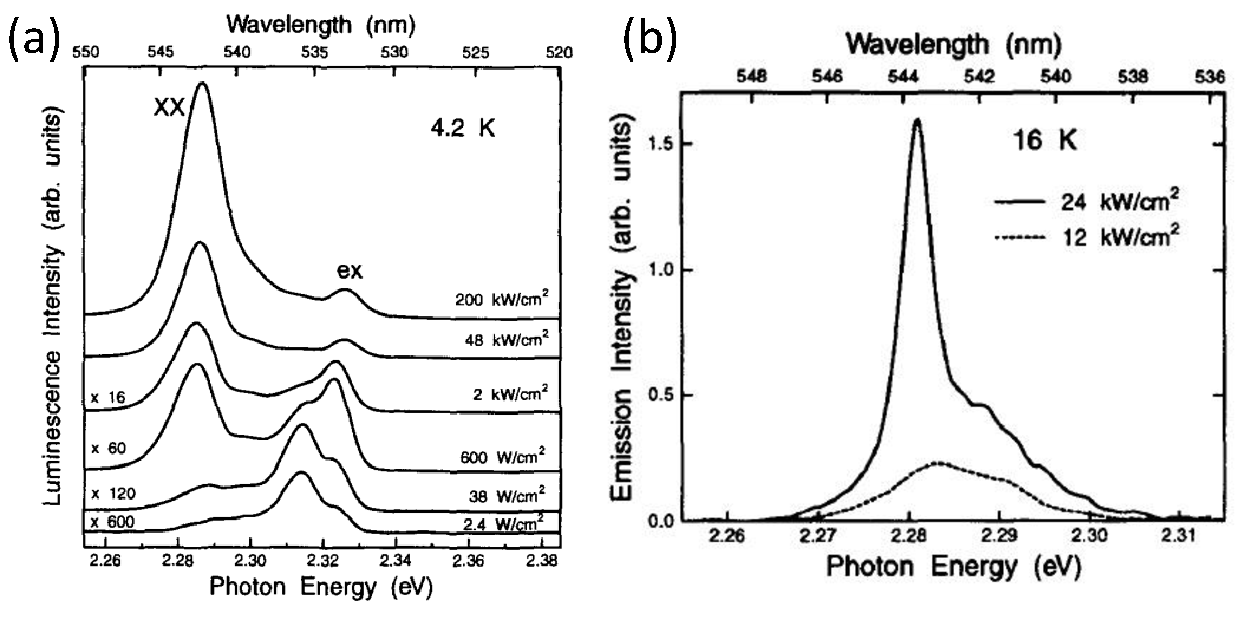
\includegraphics[width=0.8\textwidth]{Fig15}
\caption{(a) Photoluminescence spectra of $\textrm{C}_{6}$PI film excited by 337~nm nitrogen laser at 4.2K with labelled excitation intensities. Free exciton PL (labelled ex) is seen at 2.324~eV with some bound exciton PL at 2.315~eV, but the ex band dominates at low excitation. The biexciton band (labelled XX), due to the radiative recombination of a biexciton leaving behind an exciton, is located 40meV below the free exciton band. (b) Emission spectra of $\textrm{C}_{6}$PI waveguide above (24~kW/$\textrm{cm}^2$) and below (12~kW/$\textrm{cm}^2$) the lasing threshold at 4.2~K. The lasing wavelength is 543.6~nm. Reproduced from Ref.\ \cite{Kondo1998}.}
\label{2Fig15}
\end{figure}

\begin{figure}[h!]
\centering
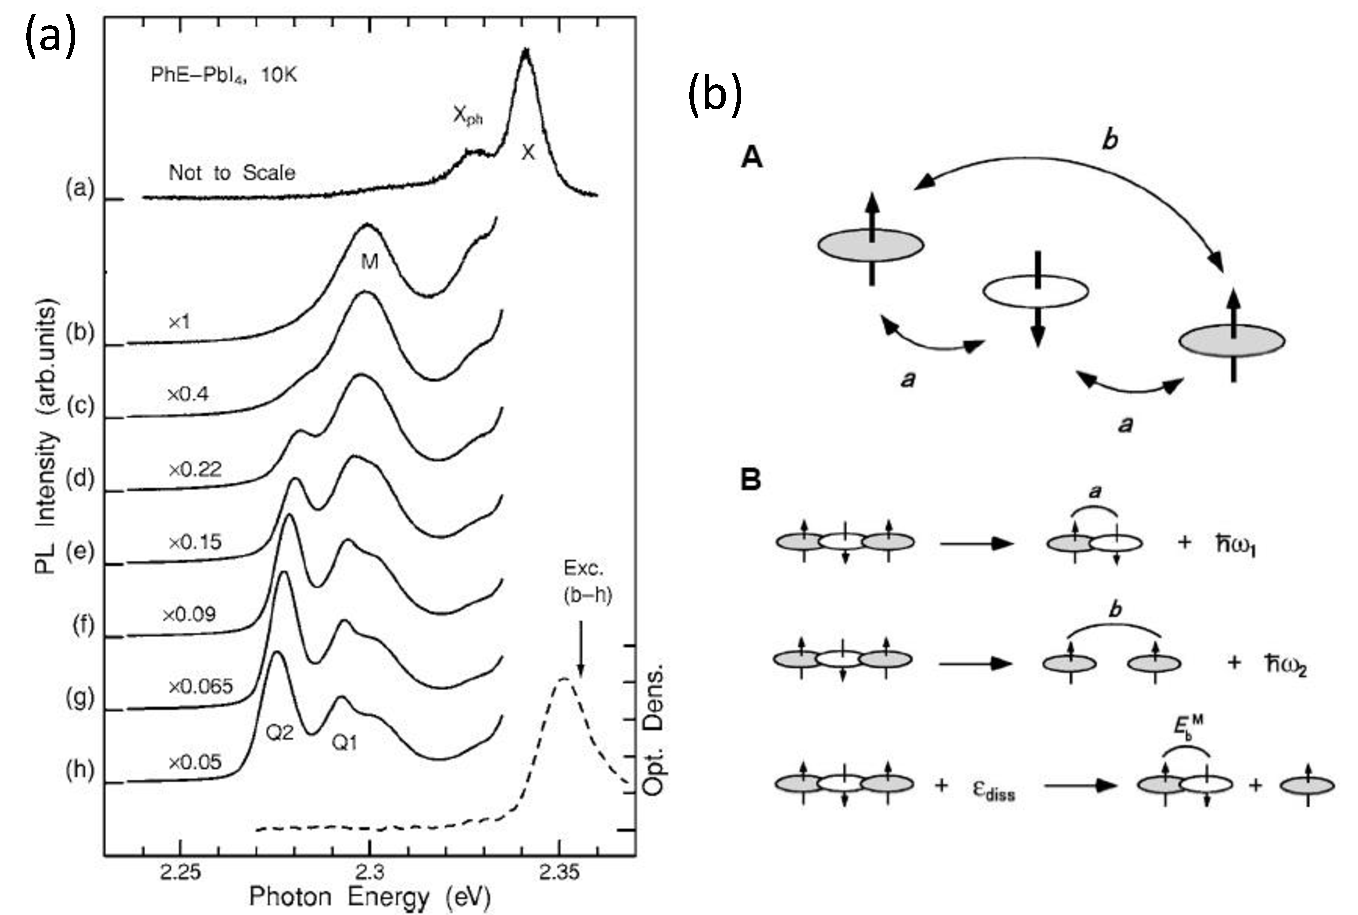
\includegraphics[width=\textwidth]{Fig16}
\caption{(a) PL spectra of PAPI at different excitation intensities and energies. (a) was excited at 2.58eV, and (b)-(h) at 2.355eV. The excitation intensities are (a) $4.6\times 10^{10}$, (b) $4.6\times 10^{12}$, (c) $1.4\times 10^{13}$, (d) $2.8\times 10^{13}$, (e) $4.6\times 10^{13}$, (f) $9.2\times 10^{13}$, (g) $1.6\times 10^{14}$, and (h) $3.2\times 10^{14}$ photons c$\textrm{m}^{-2}$. The dotted line shows the absorption spectrum. X is the free exciton band, $\textrm{X}_{\textrm{\footnotesize ph}}$ phonon sidebands, M the biexciton band, $\textrm{Q}_1$ amplified spontaneous recombination of biexcitons, and $\textrm{Q}_2$ the $\hbar \omega_2$ triexciton process in Fig.\ \ref{fig-shimizu2006-2}. (b) A) shows the triexciton model, and B) shows some likely radiative and dissociation mechanisms. For the meaning of symbols see the main text. Reproduced from Ref.\cite{Shimizu2006a}.}
\label{2Fig16}
\end{figure}

Shimizu \textit{et al.}\ observed triexciton formation in the PL spectra of PAPI. In Fig.\ \ref{2Fig16}(a), the free exciton band is labelled X, phonon sidebands $\textrm{X}_{\textrm{\footnotesize ph}}$, and M is the biexciton band. At higher excitation intensities, two other bands can be seen, labelled $\textrm{Q}_1$ and $\textrm{Q}_2$. $\textrm{Q}_1$ was assigned to the amplified spontaneous emission due biexciton recombination, and $\textrm{Q}_2$ to a triexciton process. Fig.\ \ref{2Fig16}(b) shows two of the likely radiative processes of the triexciton state, which is considered to consist of a bound state of three spin singlet excitons. $a$ denotes the interaction energy between opposite spin excitons ($<0$), $b$ denotes the interaction between same spin excitons ($>0$), $\epsilon_{\textrm{\footnotesize diss}}$ is the dissociation energy of a triexciton decaying to a biexciton and a single exciton, and $\textrm{E}_{\textrm{\footnotesize b}}^{\textrm{\footnotesize M}}$ is the binding energy of a biexciton. As $\textrm{Q}_2$ is at a lower energy than M, it can only be due to the $\hbar \omega_2$ process, although it is unclear why the $\hbar \omega_1$ process was not observed. From the data collected, it was calculated that $a$=-37.5meV, $b$=11meV, $\epsilon_{\textrm{\footnotesize diss}}$=14meV, and $\textrm{E}_{\textrm{\footnotesize b}}^{\textrm{\footnotesize M}}$=50meV \cite{Shimizu2006a}. 


\subsubsection{Dielectric confinement and the image charge effect}

Both the binding energy and oscillator strength of (transverse) excitons in 2D PbI perovskites are much larger than those in the inorganic 3D equivalent, Pb$\textrm{I}_2$ \cite{Hirasawa1994}. In materials where a sheet is sandwiched between barrier layers with lower dielectric constant $\epsilon_b$ and higher band gap, three types of confinement affect excitons. Firstly ``dielectric confinement", where the lower barrier $\epsilon_b$ reduces the effective dielectric constant of the entire structure, thus providing less shielding and giving a higher binding energy $E_b$. Secondly ``quantum confinement", where the reduction in dimensionality to 2D gives a binding energy four times larger than expected in bulk 3D material \cite{Shinada1966}. Thirdly ``mass confinement", where carrier wavefunctions extending into the barrier region lead to a larger effective mass, thus increasing the binding energy. Mass confinement depends on quantum confinement in order to determine how much of the carrier wavefunction is leaked into the barrier region, and generally only has a small effect \cite{Kumagai1989}. The interfaces between layers also act as mirrors which create an infinite series of image charges (see Fig.\ \ref{2Fig17}). Using carrier wavefunctions which fit the boundary conditions of the well, as well as self and image-charge Hamiltonians, exciton properties can be calculated. The results showed that the binding energy of excitons increase if the barrier height decreases, the excitons have larger effective mass in carrier region, or the barrier regions have a smaller dielectric constant \cite{Kumagai1989}. Muljarov \textit{et al.}\ found that the potentials created due to the image charge effect causes charges in the inorganic layers to be repelled from the interface, whereas charges in the organic layers are attracted to the interface \cite{Muljarov1995}.

\begin{figure}[ht]
\centering
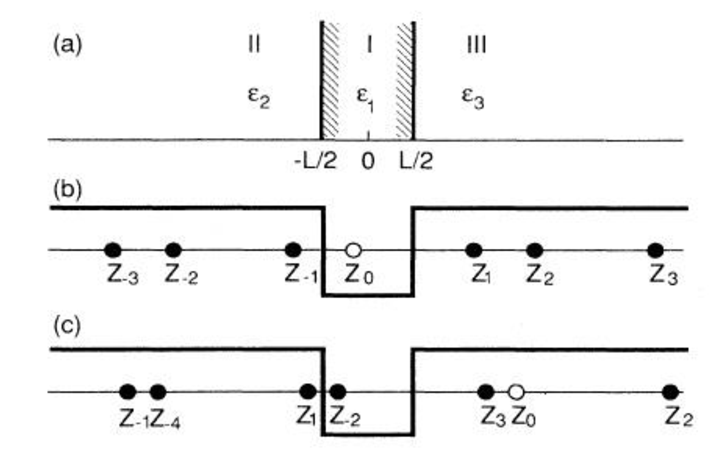
\includegraphics[width=0.8\textwidth]{Fig17}
\caption{(a) Generalised description of quantum well (region I) and barriers (regions II and III). (b) and (c) show the positions of initial charges (white circle) and image charges created (black circles) due to interfaces. In (b) the initial charge is in the well region, whereas in (c) it is in the barrier region. Reproduced from Ref.\ \cite{Kumagai1989}.}
\label{2Fig17}
\end{figure}


\subsubsection{Pressure induced changes}
Fig.\ \ref{2Fig18} shows how the absorption and PL spectra of $\textrm{C}_8$PI changes when pressure is applied to the material in a diamond cell. Both sets of spectra show that the exciton energy decreases as the pressure increases, since a reduction in Pb-I distance leads to an increase in the energy of the antibonding valence band, with the non-bonding conduction band less affected \cite{Matsuishi2004}. After a phase transition at 12GPa, absorption spectra show much broader ``tails" that can be described by Urbach's rule, and correlates with the disappearance of exciton signatures in PL spectra. Fig.\ \ref{2Fig18}(c) shows changes in PL intensity on the up-stroke (pressure increasing from ambient) and down-stroke (pressure decreasing down to ambient). A large hysteresis is observed, with PL intensities significantly smaller on the down-stroke than on the up-stroke with. The results suggest that defects may have been created with the increase in pressure. As excitons above and below the phase transition seem to involve different electronic states, it has been postulated that the band structure of $\textrm{C}_8$PI is such that exciton formation involves a direct transition below 12GPa, which changes to an indirect transition above 12GPa \cite{Matsuishi2001}. The same experiment was performed on $\textrm{C}_4$PI with similar results. In $\textrm{C}_4$PI the phase transition occurred around 10GPa, although some residue of the free exciton band was still seen at 11.2GPa. The difference in transition pressures suggests that the change in exciton energy is at least in part due to a transition in the organic molecules \cite{Matsuishi2004}.
\begin{figure}[h!]
\centering
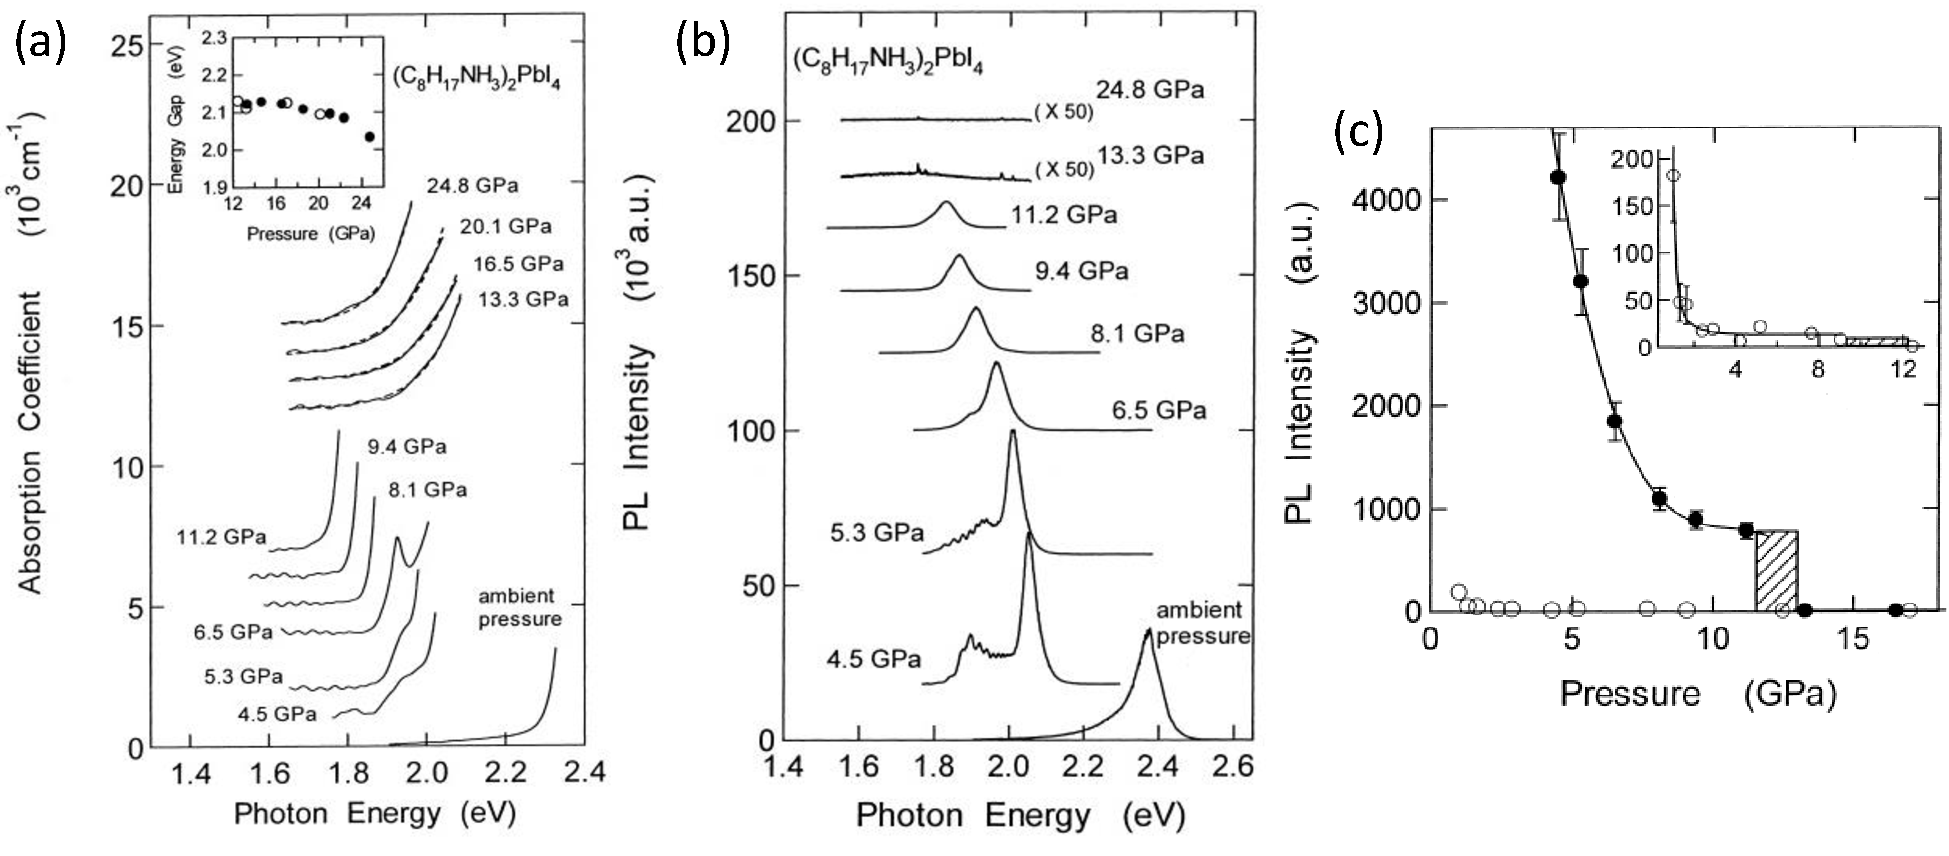
\includegraphics[width=\textwidth]{Fig18}
\caption{(a) Absorption, and (b) PL spectra of $\textrm{C}_8$PI under labelled pressure. Exciton energies decrease with increasing pressure, and a phase transition is seen at around 12GPa. The sidebands seen at 4.5 and 5.3GPa spectra are possibly due to bound excitons. The inset of (a) shows the band gap as calculated using Urbach's rule above phase transition.  (c) PL intensity against applied pressure for the up-stroke (black circles) and down-stroke (white circles). The shaded box indicates the position of the phase transition. A large hysteresis can be seen as the up-stroke may create defects in the crystal. Reproduced from Ref.\ \cite{Matsuishi2001}.}
\label{2Fig18}
\end{figure}


\subsection{Influence of organic molecules}
How an organic molecule fits into the MQW structure can change the distortion of octahedra, the I-Pb-I bond angle, or the interlayer I-I coupling, all of which lead to a change in the electronic structure \cite{Sourisseau2007}.

Pb-I-Pb bond angles (i.e.\ how flat the inorganic sheet is) has a large effect on the band gap of perovskites. Experimental results show that bond angles closer to $180^{\circ}$ (undistorted octahedra) lead to smaller band gaps, which agrees with extended Huckel tight-binding calculations used to evaluate band structures of PbI perovskites (results are seen in Fig.\ \ref{2Fig19}). Although the band gaps are underestimated using this model, the overall correlation between I-Pb-I angle and electronic energy levels are correct \cite{Pradeesh2009}.
\begin{figure}[ht]
\centering
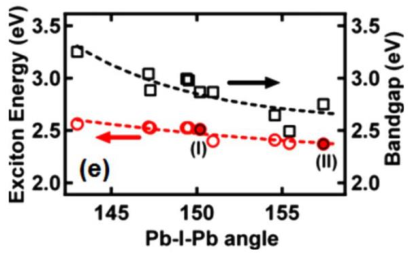
\includegraphics[width=0.6\textwidth]{Fig19}
\caption{Variation in exciton energy (red) and band gap (black) with I-Pb-I angles calculated using extended Huckel tight binding calculations.  Filled in circles represent PL maxima of labelled $\textrm{C}_{12}$PI phases. The calculations show that exciton and band gap energies both decrease as the Pb-I-Pb bond angle increases. Reproduced from Ref.\ \cite{Pradeesh2009}.}
\label{2Fig19}
\end{figure}

2,$2^{'}$-biimidazole ($\textrm{C}_6\textrm{H}_6\textrm{N}_4$) was incorporated into the perovskite structure to form $(\textrm{C}_6\textrm{H}_8\textrm{N}_4)\textrm{PbI}_4$, and the organic molecules can be doubly protonated to $2^+$, or accept two electrons and delocalise the charge across the entire molecule. Since the corrugation of the organic layer is increased if there are strong hydrogen bonds between the organic and inorganic moieties, the weak hydrogen bonds in $(\textrm{C}_6\textrm{H}_8\textrm{N}_4)\textrm{PbI}_4$ lead to flatter sheets, and thus a smaller band gap \cite{Tang2001}. Similarly in $(\textrm{HO(CH}_2)_2\textrm{NH}_3)_2\textrm{PbI}_4$, where the -OH group is able to hydrogen bond with neighbouring -$\textrm{NH}_3$ groups or iodine atoms. The extra interactions do not just weaken the $\textrm{NH}_3$-I hydrogen bonds, but provide a channel for stronger electronic coupling between inorganic layers, leading to a smaller band gap \cite{Mercier2004}.

For a perovskite of form $(\textrm{R-(CH}_2)_n\textrm{NH}_3)_2\textrm{PbI}_4$, for each -R there appears to be a optimal $n$ that leads to an arrangement that provides the best PL efficiency. In general PL efficiencies are better if the inorganic sheets are close to flat, so as well as hydrogen bonding considerations, the best organic molecules have an -R group that is not too big or small to fit in the spaces between iodine atoms, causing the sheet to deform. Similarly if -R is flexible (e.g.\ alkyl rather than phenyl), then molecules can fit into interlayer spaces without too much deformation of inorganic sheets \cite{Zhang2009}.

As well as effects on the structural leading to optical changes, properties of the organic ligand can be be incorporated into the material. For example when chiral organic molecules are used, the perovskite also exhibits optical activity \cite{Teshima2003}. Similarly tuning the band gap of the organic constituents can lead to charge and energy transfer between the organic and inorganic layers \cite{Kawabata2009, Mitzi1999a, Braun1999}.

\subsection{Applications}
\subsubsection{Microcavities and photonic crystals}
Strong coupling has been observed between PAPI excitons and cavity modes in a distributed feedback microcavity at room temperature \cite{Fujita1998, Fujita1999, Fujita2000}. The cavity consists of a quartz substrate with PAPI spin coated into the spaces as shown in Fig.\ \ref{2Fig20}(a) to form parallel wires, and an overcoat of polystyrene added to prevent the degradation of PAPI films. The grating pitch ($\Gamma$) was around 0.7$\mu$m, the depth ($h$) 0.3$\mu$m, PAPI thickness 0.03$\mu$m, and polystyrene thickness 0.5$\mu$m; overall the grating had an area of around 1.5$\times$1.5mm. Inside the cavity light is modulated in the $x$ direction, homogeneous in the $y$ direction, and confined in the $z$ direction \cite{Fujita1999}. When the incident beam is at normal incidence, it is expected that PAPI excitons will couple strongly to the fourth order cavity resonance and form new eigenstates (``cavity polaritons"). Using a variety of grating sizes from 0.62 to 0.72$\mu$m, transmission spectra showed that the upper and lower polariton branches exhibited anti-crossing behaviour, as expected for strongly coupled modes. Due to the large exciton oscillator strength, the mode splitting was around 100meV, larger than the 9meV observed in GaAs systems in Fabry-Perot microcavities \cite{Fujita1998}. A strong enhancement of PL intensity of the lower branch polariton is seen if the standing wave cavity mode is in resonance with PAPI excitons, in this case when $\Gamma=0.68\mu$m \cite{Fujita1999}. No signature of the upper polariton branch was seen since in thermodynamic equilibrium the upper branch would expect to be less populated, however the polariton lifetime may not be long enough for equilibrium to occur. Other suggestions have included a relaxation of the upper branch polaritons towards uncoupled excitonic states, or fast emission of photons between the upper and lower polariton branches \cite{Lanty2008}. It was thought that the PAPI rods oscillating in phase due to strong coupling with cavity modes at resonance would lead to a macroscopic polarisation and ultrafast resonance, however the polariton lifetime was actually 8ps longer with a grating structure at 40~K. It is possible that this is due to excitons with large wave vectors that cannot couple to the outside without the help of the reciprocal lattice vector \cite{Fujita2000}. 

Strong coupling between cavity and PAPI exciton modes were also observed in the Fabry-Perot microcavity [Fig.\ \ref{2Fig20}(b)] \cite{Brehier2006, Lanty2008}. By adjusting the position of the perovskite layer in the microcavity, the coupling between exciton and photon modes could be controlled, and the splittings seen were between 130-190~nm. Similar CHPI microcavities were constructed and showed splittings of 130meV for a $5\lambda/4$ metal-air microcavity, and of 160meV for a $7\lambda/4$ metal-metal microcavity \cite{Pradeesh2009b}.

\begin{figure}[h!]
\centering
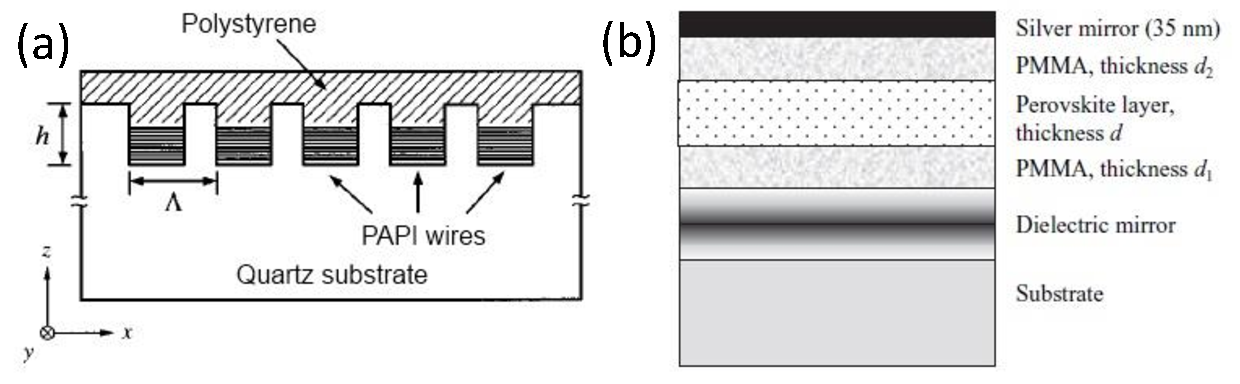
\includegraphics[width=\textwidth]{Fig20}
\caption{Schematic of (a) a distributed feedback microcavity, (b) Fabry-Perot microcavity, (c) 2D photonic crystal. In (a) and (c) $\Gamma$ represents the grating pitch, $h$ the grating depth, $\textrm{d}_\textrm{\footnotesize PS}$ the height of the polystyrene layer. $\theta$, the angle of incident light, is also labelled. (a) reproduced from Ref.\ \cite{Fujita1998}, (b) from \cite{Lanty2008}, (c) from \cite{Ishi-Hayase2003}.}
\label{2Fig20}
\end{figure}

Strong exciton-photon coupling was also seen in a photonic crystal of silica microspheres infiltrated with PAPI (silica opal) \cite{Sumioka2001}. A face centred cubic lattice of silica microspheres with 3D channel voids was created, and a solution of PAPI and DMF were introduced into continuous spaces through capillary forces. The structure was then left for 12hrs at $25^{\circ}$C for the solvent to evaporate. Fig.\ \ref{2Fig21}(b) shows the reflectivity spectra for a range of incidence angles $\theta$. When $\theta=10^{\circ}$, the band near 2.13eV is attributed to the stop band of the photonic crystal, and the band near 2.4eV to excitons in PAPI. At larger angles the stop band blue shifts and asymptotically approaches the almost constant exciton band. Above $\theta=35^{\circ}$ another band appears on the higher energy side of the exciton band. The solid black line in Fig.\ \ref{2Fig21}(c) shows a plot of the expected stop band energy as a result of the photonic structure of a silica opal with a PAPI filling fraction ($f_{\textrm{\footnotesize PAPI}}$) of 0.06, the dashed black line shows the energy of an exciton for a PAPI sample in free space, and the black circles show experimental peak values from Fig.\ \ref{2Fig21}(b). The silica opal clearly demonstrates anticrossing behaviour, indicating a strong coupling between the stop band (photon mode) and the exciton mode of PAPI, with a Rabi splitting of 240meV. However there is an exciton peak that seems largely unaffected by the photon modes, and this may be due to some of the bulk PAPI on the surface of the silica opal remaining, or an open photonic gap in the silica opal which leads to insufficient photon confinement, and thus limiting the exciton-photon coupling. Similar strong coupling was seen in the 2D photonic crystal shown in Fig.\ \ref{2Fig20}(c), where the anticrossing splitting was also 100meV \cite{Ishi-Hayase2003}. 
\begin{figure}[h!]
\centering
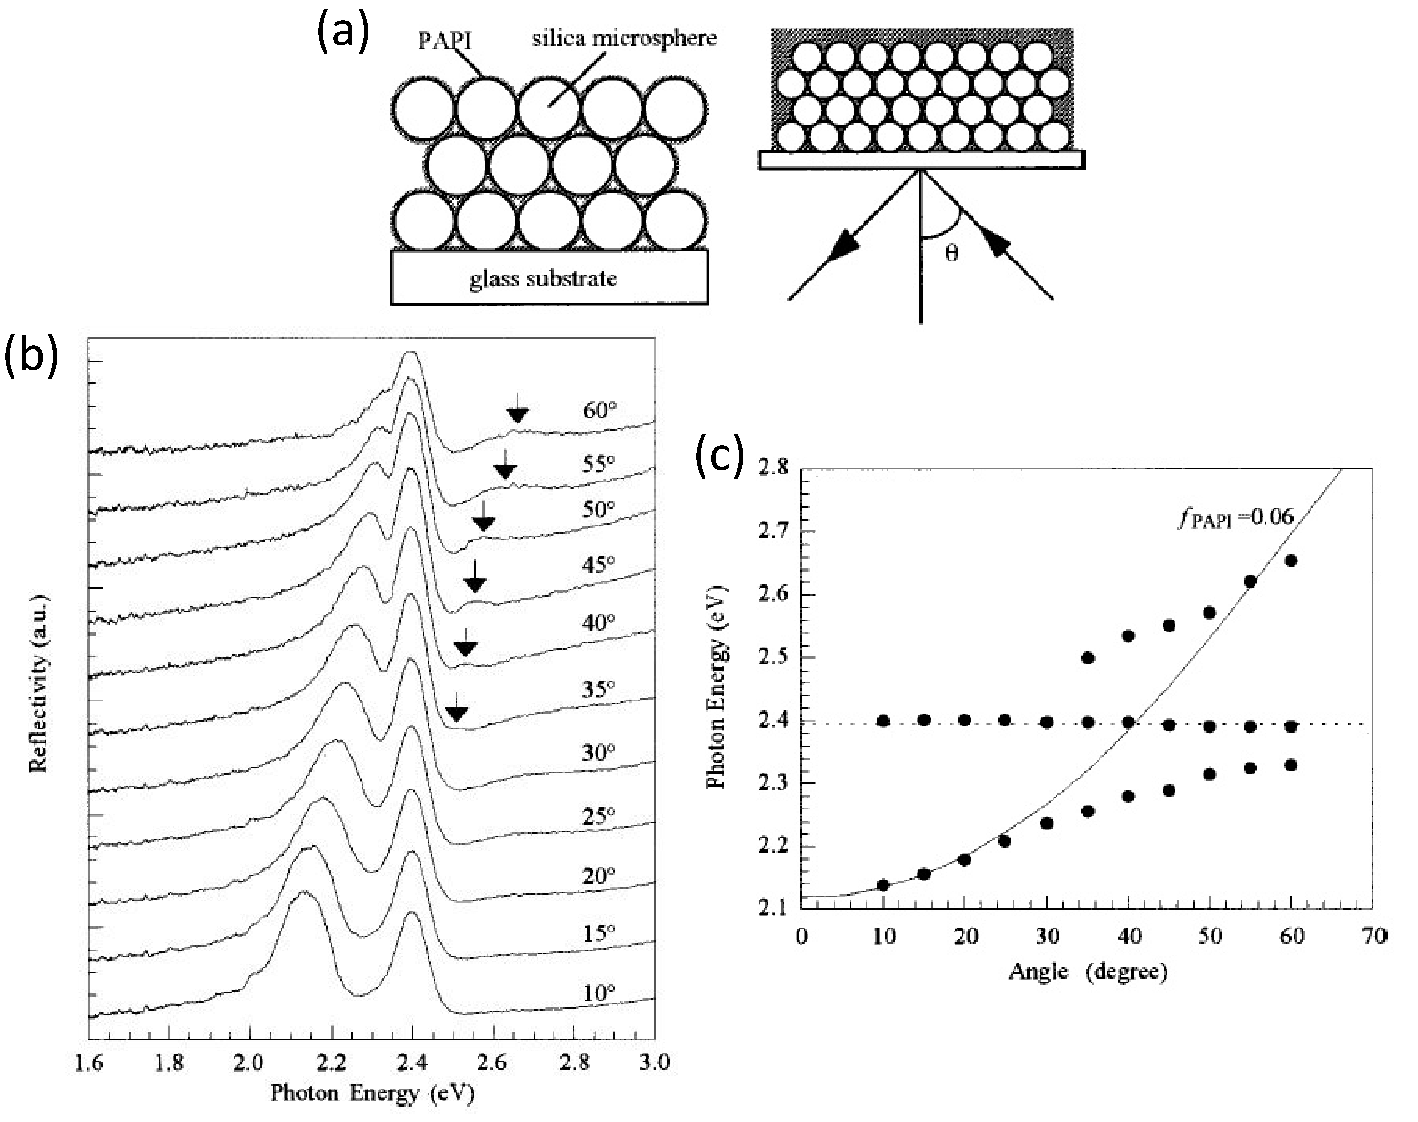
\includegraphics[width=\textwidth]{Fig21}
\caption{(a) Schematic of the structure of the silica opal infiltrated with PAPI film formed on a glass substrate. $\theta$, the angle of incident light, is also shown. (b) Reflection spectra recorded for a range of $\theta$ values, displaced vertically for clarity but plotted on the same scale. The lower polariton branch peaks asymptotatically approaches the exciton peaks at 2.4eV, and small upper polariton branch peaks can be seen at high angles. (c) Peak energies (black circles) against observation angle. The solid black line is the theoretical stop gap energy from Bragg's law, and the dashed black line is the exciton energy of PAPI in free space. Anticrossing behaviour can clearly be observed, and unaffected exciton peaks may be due to some bulk PAPI remaining on the photonic crystal. Reproduced from Ref.\ \cite{Sumioka2001}.}
\label{2Fig21}
\end{figure}

\subsubsection{Optoelectronic devices}
Era \textit{et al.}\ used spin coated PAPI to make an electroluminescent (EL) device. Fig.\ \ref{2Fig22}(a) contains a schematic of the device, consisting of an indium-tin-oxide (ITO) anode, MgAg cathode, and oxadiazole (OXD7) was used as the electron transport layer. As the device is driven, electrons in the OXD7 layer are injected smoothly into the PAPI layer as there is no energy barrier [Fig.\ \ref{2Fig22}(b)]. On the other hand, holes injected into PAPI will remain at the PAPI/OXD7 interface due to the barrier potential created by the large OXD7 ionisation potential. Electrons and holes are trapped in the PAPI layer, then recombine to provide luminescence. When driven at liquid nitrogen temperatures, the EL intensity reached a luminescence of more than 10000cd$\textrm{m}^2$ at a current density of 2A$\textrm{cm}^{-2}$ and voltage of 24V. The emission peak at 520nm has a narrow bandwidth, and is very similar to the PL spectrum. However the EL efficiency at room temperature is much smaller than that at liquid nitrogen temperatures, and is mainly caused by thermal ionisation of excitons \cite{Era1994}.
\begin{figure}[h!]
\centering
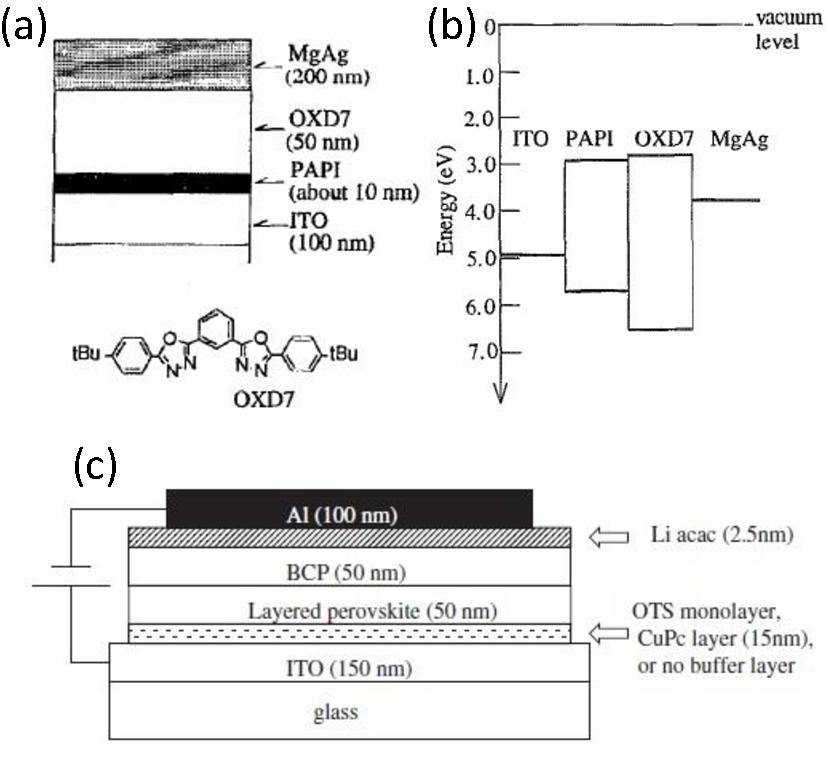
\includegraphics[width=0.8\textwidth]{Fig22}
\caption{(a) Schematic of the EL device (top) and the molecular structure of OXD7 (bottom). (b) Energy level diagram of EL device. Electrons are smoothly injected from OXD7 to PAPI, however holes remain at the PAPI/OXD7 interface due to large barrier potential. Reproduced from Ref.\cite{Era1994}.}
\label{2Fig22}
\end{figure}

Hattori \textit{et al.}\ made similar EL devices using both PAPI, CHPI, and PBPI ($\textrm{(C}_6\textrm{H}_5\textrm{C}_4\textrm{H}_8\textrm{NH}_3)_2\textrm{PbI}_4$). The authors found that CHPI and PBPI both have much higher PL efficiencies than PAPI. While the EL spectra look very similar to the PL spectra [Fig.\ \ref{2Fig23}], the PBPI device had the lowest external quantum efficiency $\eta_{ext}$ (number of emitted photons/number of electrons) and CHPI the highest. The PBPI device was also much more resistive than the others, with current density around two orders of magnitude less than other devices at same voltage. Both the resistance and the low EL efficiency are probably due to the larger alkyl chain in the organic molecule preventing carrier transport. The external efficiency of the CHPI device was comparable to the highest efficiency reported in EL devices reported at that stage \cite{Hattori1996}.

\begin{figure}[h!]
\centering
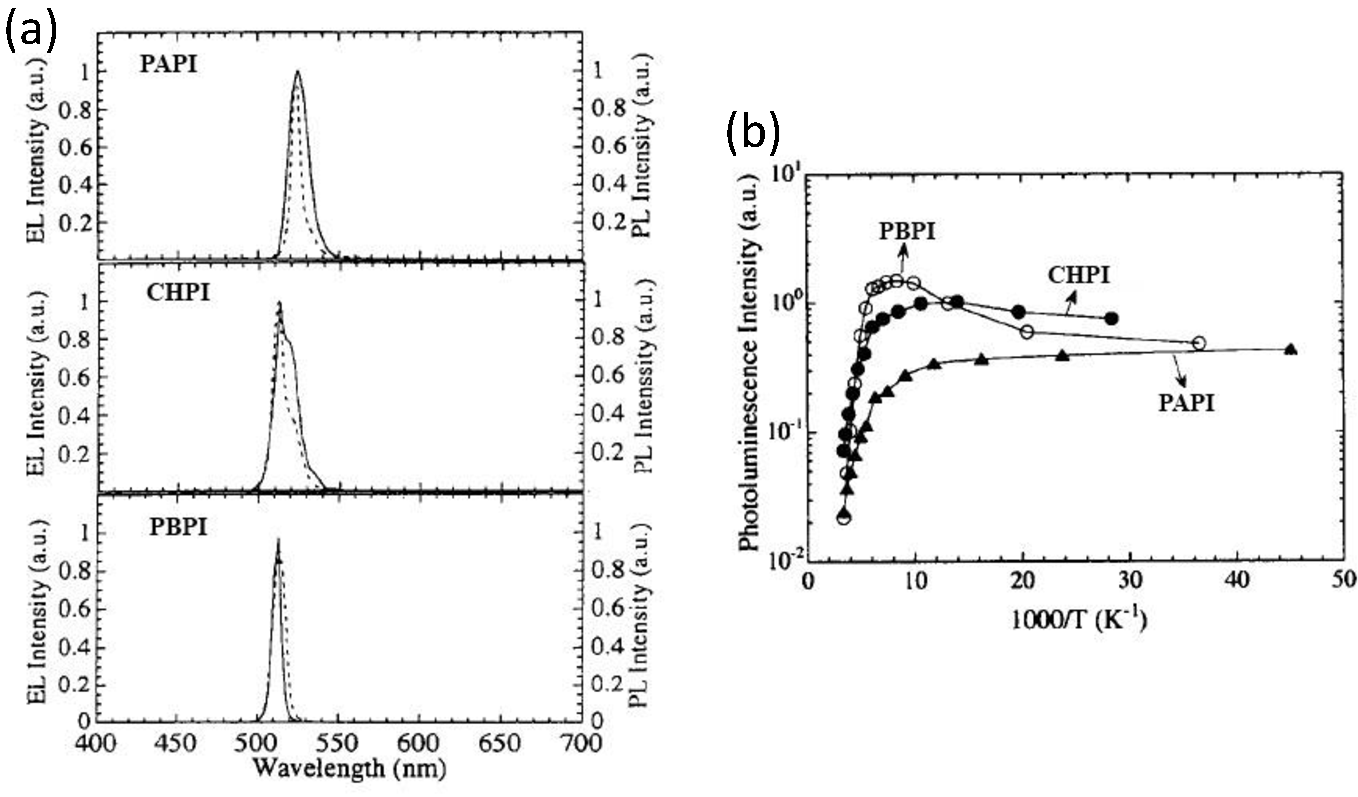
\includegraphics[width=\textwidth]{Fig23}
\caption{(a) Integrated PL intensity of CHPI, PAPI, and PBPI thin film samples as a function of temperature. (b) EL (solid lines) and PL (dotted lines) spectra of the labelled perovskite. EL devices were made as shown in Fig.\ \ref{2Fig22}(a), and driven at 110K. PL spectra were recorded using thin film samples at 110K. Although the EL and PL spectra are very similar for all three compounds, the CHPI device had the highest EL efficiency, while PBPI had the worst. Reproduced from Ref.\ \cite{Hattori1996}.}
\label{2Fig23}
\end{figure}

Matsushima \textit{et al.}\ used PAPI to create LEDs (schematic shown in Fig.\ \ref{2Fig24}). PAPI films were deposited onto an OTS coated, CuPc coated, or bare substrate (OTS=octadecyltrichlorosilane, CuPc=Cu pthalocyanine), then annealed for 20~mins at $100^{\circ}$C. PAPI films on substrates with an OTS monolayer were more crystalline and had larger absorption intensities compared to bare glass substrates, however films on CuPc covered substrates had the smallest surface roughness. Driven at 105~K, CuPc-coated samples had the best EL efficiency due to a lowering of the hole injection barrier at the ITO/PAPI interface, and also due to smaller leakage currents as a result of smaller surface roughness of PAPI films \cite{Matsushima2005}.
\begin{figure}[h!]
\centering
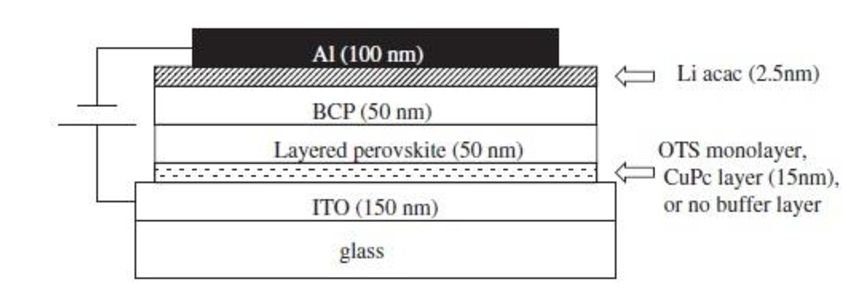
\includegraphics[width=0.8\textwidth]{Fig24}
\caption{Schematic of the LED made used PAPI films. PAPI was spin coated on either an OTS coated glass substrate, a CuPc coated glass substrate, or a bare glass substrate. Reproduced from Ref.\ \cite{Matsushima2005}.}
\label{2Fig24}
\end{figure}

The processability of hybrid perovskites from solution make them ideal materials for use in optoelectronic devices. The conductivity of SnI-based perovskites have been investigated, and show that while 2D layered structures are semiconducting, the 3D perovskite structure is a low-carrier density p-type metal with a corresponding increase in the conductivity \cite{Mitzi1994}. Thin film transistors have also been produced from the 2D perovskite, with carrier mobilities of up to 1.4\,cm$^2$/Vs, better than that of amorphous silicon, on-off ratio $>1000$, and current densities $>400$\,A/cm$^2$ \cite{Mitzi2002b, Mitzi2001d, Kagan199a}.

\subsubsection{Scintillators}
Scintillators need to convert radiation energy into photo-emission for the purpose of detecting ionising radiation. They need to have a short luminescence decay time constant in order to react quickly, high resistance to radiation damage, and high efficiency so that a suitable number of photons are created per unit radiation energy of absorbed \cite{Shibuya2002}. Many efficient scintillators (e.g.\ NaI:TI, CsI:Na) have decay times of 200ns or more, whereas fast scintillators (e.g.\ Ba$\textrm{F}_2$, CsF) have low light yields of less than 2000~photons per MeV \cite{Kengo2002}. In order to test its suitability, $\textrm{C}_6$PI crystals were bombarded by an ultra-short electron beam with pulse width of 1-2ps, generated by a 35MeV linear accelerator. It was found that $\textrm{C}_6$PI had a decay constant of 45ps at room temperature \cite{Kengo2002}. The 3D extension of 2D perovskites, $\textrm{CH}_3\textrm{NH}_3\textrm{PbBr}_3$ was also tested, and the 2D perovskite had a faster decay time as quantum confinements means carrier wavefunctions overlap, giving higher likelihood of decay.

Shibuya \textit{et al.}\ used different dosages of 2MeV protons to test $\approx250$nm $\textrm{C}_6$PI thin films \cite{Shibuya2002}. Radiation-induced emission spectra showed that the exciton peak did not change position during bombardment, and no additional peaks appeared at any radiation dosage. Three decay components were found: one with decay constant 0.39~ns due to free exciton recombination, then two more with constants of 3.8 and 16~ns due to trapped excitons, with decay constants depending on defect density. Emission intensities of $\textrm{C}_6$PI excitons attenuated with increased radiation, but the radiation hardness was still enough for practical use. From these results, $\textrm{C}_6$PI would be a good candidate for scintillator use due to the stability of excitons at room temperature, ease of processing, fast response due to short exciton lifetime, no shift in spectrum due to radiation, and inclusion of high atomic number element of Pb in order to detect low linear energy transfer radiation such as X-rays \cite{Shibuya2004}. 

\section{Conclusions}
Excitons, bound hydrogen atom-like systems of electrons and holes, produce strong optical signatures in semiconductors. Such effects can be enhanced as a result of a reduction in dimensionality. PbI perovskites are naturally self-assembling materials that create a MQW structure, and whose optical properties are dominated by the excitons produced in the inorganic layers even at room temperature. The great flexibility of the perovskite structure, as well as its processability, provide tunability for use of the material in device applications.